% Options for packages loaded elsewhere
\PassOptionsToPackage{unicode}{hyperref}
\PassOptionsToPackage{hyphens}{url}
\PassOptionsToPackage{dvipsnames,svgnames,x11names}{xcolor}
%
\documentclass[
  12pt,
]{book}
\usepackage{amsmath,amssymb}
\usepackage{lmodern}
\usepackage{iftex}
\ifPDFTeX
  \usepackage[T1]{fontenc}
  \usepackage[utf8]{inputenc}
  \usepackage{textcomp} % provide euro and other symbols
\else % if luatex or xetex
  \usepackage{unicode-math}
  \defaultfontfeatures{Scale=MatchLowercase}
  \defaultfontfeatures[\rmfamily]{Ligatures=TeX,Scale=1}
\fi
% Use upquote if available, for straight quotes in verbatim environments
\IfFileExists{upquote.sty}{\usepackage{upquote}}{}
\IfFileExists{microtype.sty}{% use microtype if available
  \usepackage[]{microtype}
  \UseMicrotypeSet[protrusion]{basicmath} % disable protrusion for tt fonts
}{}
\makeatletter
\@ifundefined{KOMAClassName}{% if non-KOMA class
  \IfFileExists{parskip.sty}{%
    \usepackage{parskip}
  }{% else
    \setlength{\parindent}{0pt}
    \setlength{\parskip}{6pt plus 2pt minus 1pt}}
}{% if KOMA class
  \KOMAoptions{parskip=half}}
\makeatother
\usepackage{xcolor}
\usepackage[margin = 2cm]{geometry}
\usepackage{longtable,booktabs,array}
\usepackage{calc} % for calculating minipage widths
% Correct order of tables after \paragraph or \subparagraph
\usepackage{etoolbox}
\makeatletter
\patchcmd\longtable{\par}{\if@noskipsec\mbox{}\fi\par}{}{}
\makeatother
% Allow footnotes in longtable head/foot
\IfFileExists{footnotehyper.sty}{\usepackage{footnotehyper}}{\usepackage{footnote}}
\makesavenoteenv{longtable}
\usepackage{graphicx}
\makeatletter
\def\maxwidth{\ifdim\Gin@nat@width>\linewidth\linewidth\else\Gin@nat@width\fi}
\def\maxheight{\ifdim\Gin@nat@height>\textheight\textheight\else\Gin@nat@height\fi}
\makeatother
% Scale images if necessary, so that they will not overflow the page
% margins by default, and it is still possible to overwrite the defaults
% using explicit options in \includegraphics[width, height, ...]{}
\setkeys{Gin}{width=\maxwidth,height=\maxheight,keepaspectratio}
% Set default figure placement to htbp
\makeatletter
\def\fps@figure{htbp}
\makeatother
\setlength{\emergencystretch}{3em} % prevent overfull lines
\providecommand{\tightlist}{%
  \setlength{\itemsep}{0pt}\setlength{\parskip}{0pt}}
\setcounter{secnumdepth}{5}
\ifLuaTeX
\usepackage[bidi=basic]{babel}
\else
\usepackage[bidi=default]{babel}
\fi
\babelprovide[main,import]{spanish}
% get rid of language-specific shorthands (see #6817):
\let\LanguageShortHands\languageshorthands
\def\languageshorthands#1{}
\usepackage{setspace}
%\linespread{1.5}
%\usepackage{tikz}
%\usetikzlibrary{shapes,arrows}
\usepackage{pdflscape}
\newcommand{\blandscape}{\begin{landscape}}
\newcommand{\elandscape}{\end{landscape}}
\renewcommand{\thesection}{\Roman{section}}
\renewcommand{\thesubsection}{\Alph{subsection}}
\usepackage{booktabs}
\usepackage{amsthm}
\makeatletter
\def\thm@space@setup{%
  \thm@preskip=8pt plus 2pt minus 4pt
  \thm@postskip=\thm@preskip
}
\makeatother
\usepackage[spanish, spanishkw, onelanguage, linesnumbered, amsmath]{}
\ifLuaTeX
  \usepackage{selnolig}  % disable illegal ligatures
\fi
\usepackage[]{natbib}
\bibliographystyle{apalike}
\IfFileExists{bookmark.sty}{\usepackage{bookmark}}{\usepackage{hyperref}}
\IfFileExists{xurl.sty}{\usepackage{xurl}}{} % add URL line breaks if available
\urlstyle{same} % disable monospaced font for URLs
\hypersetup{
  pdftitle={Diseño y análisis estadístico en las encuestas de hogares de América Latina},
  pdfauthor={Andrés Gutiérrez},
  pdflang={es},
  colorlinks=true,
  linkcolor={blue},
  filecolor={Maroon},
  citecolor={Blue},
  urlcolor={Blue},
  pdfcreator={LaTeX via pandoc}}

\title{Diseño y análisis estadístico en las encuestas de hogares de América Latina}
\author{Andrés Gutiérrez\footnote{Experto Regional en Estadísticas Sociales - Comisión Económica para América Latina y el Caribe (CEPAL) - \href{mailto:andres.gutierrez@cepal.org}{\nolinkurl{andres.gutierrez@cepal.org}}}}
\date{2022-09-28}

\begin{document}
\maketitle

{
\hypersetup{linkcolor=}
\setcounter{tocdepth}{1}
\tableofcontents
}
\listoffigures
\listoftables
\hypertarget{prefacio}{%
\chapter*{Prefacio}\label{prefacio}}
\addcontentsline{toc}{chapter}{Prefacio}

\begin{figure}

\includegraphics[width=100px]{Pics/CClicence} \caption{Licencia de Creative Commons}\label{fig:unnamed-chunk-1}
\end{figure}

La versión online de este libro está licenciada bajo una \href{http://creativecommons.org/licenses/by-nc-sa/4.0/}{Licencia Internacional de Creative Commons para compartir con atribución no comercial 4.0}.

La coordinación sustantiva de la colección Metodologías de la CEPAL está a cargo de Rolando Ocampo, Director de la División de Estadísticas de la Comisión Económica para América Latina y el Caribe (CEPAL).

Esta publicación es el resultado de un proceso de varios años de investigación e interacción con los países miembros en diversas asistencias técnicas concernientes con el diseño, rediseño y análisis posterior de las encuestas de hogares. Dicho proceso fue llevado a cabo por la División de Estadísticas de la CEPAL, bajo la coordinación de Rolando Ocampo, Director de la División de Estadísticas y de Xavier Mancero, Jefe de la Unidad de Estadísticas Sociales. La redacción del documento estuvo a cargo de Andrés Gutiérrez, Asesor Regional en Estadísticas Sociales de la CEPAL.

Las metodologías presentadas en este documento se han beneficiado de los valiosos aportes y sugerencias de funcionarios de la CEPAL, así como del personal de las Oficinas Nacionales de Estadística de los países beneficiarios de las asistencias técnicas durante los años entre 2017 y 2022. El autor agradece a Simone Ceccini y a Xavier Mancero por la lectura detallada de este documento y sus comentarios.

\hypertarget{resumen}{%
\chapter*{Resumen}\label{resumen}}
\addcontentsline{toc}{chapter}{Resumen}

Las encuestas de hogares son un instrumento necesario para realizar seguimiento a un conjunto amplio de indicadores requeridos para el diseño y evaluación de las políticas públicas. Las encuestas de hogares que se implementan en América Latina son de tipo y características diversas. Aunque los conceptos y procesos para su diseño y análisis guardan similitudes, este documento se enfoca principalmente en los procesos referidos a las encuestas de empleo y de propósitos múltiples, con las que los países estiman los principales indicadores relacionados con el mercado laboral, el nivel y distribución de ingresos y la condición de pobreza y las principales características sociodemográficas de la población. Se realiza un recorrido por los diferentes diseños de muestreo, las metodologías más usadas en la selección de las muestras y las estrategias de estimación de los parámetros de interés. También se revisan las técnicas utilizadas para medir el error de muestreo y los métodos disponibles para encarar desafíos como la ausencia de respuesta y la desactualización de los marcos de muestreo.

\textbf{UNBIS Keywords}. Encuestas por muestreo, encuestas de hogares, indicadores socioeconómicos.

\hypertarget{introducciuxf3n}{%
\chapter{Introducción}\label{introducciuxf3n}}

Este documento pretende revisar algunas de las metodologías más usadas por las ONE de América Latina en cuanto al diseño y análisis estadístico de las encuestas de hogares y puede servir de guía técnica a los estadísticos de la región que se encuentran involucrados en los procesos técnicos de este tipo de encuestas. De la misma forma, este documento considera conjuntamente los dos principales momentos de las encuestas: el diseño y el análisis. Nótese que estos momentos están escindidos por el levantamiento de la información en campo y parten la realización de la encuesta en dos. Los lectores que están familiarizados con la investigación social a través de las encuestas de hogares encontrarán que estas operaciones estadísticas se planean teniendo en cuenta muchos pormenores que podrían suceder en campo. Es por esto que el trabajo de los investigadores en las ONE es que el mismo diseño que se planificó se logre plasmar en la información recolectada en la de base de microdatos de las encuestas. En este segundo momento es cuando se debe asegurar que lo que se planificó efectivamente sea incorporado en el análisis de esta información.

Desde esta perspectiva, este documento se aborda en tres partes sustantivas que definen la planeación y el análisis de la mayoría de las encuestas de hogares en América Latina y el Caribe. La primera parte se refiere a la planeación de una encuesta y a la definición del diseño estadístico, que comprende - entre otras cosas - la generación de una medida de probabilidad discreta que soportará la inferencia basada en el principio de representatividad. En esta parte se aborda con más detalle los elementos básicos que se consideran por lo regular en los diseños de las encuestas de hogares. Un aspecto relevante es que, si bien este documento considera que las encuestas de hogares tienen muchos elementos en común, diferencia de forma cuidadosa las particularidades de cada tipo de encuesta. Por ejemplo, se trata el tema del diseño de las encuestas rotativas y se profundiza en los diferentes parámetros que se pueden considerar en este tipo de operaciones; asimismo, describe las características metodológicas que se deben considerar al momento de diseñar la encuesta y revisa los conceptos esenciales que determinarán el tipo de aplicación que se debe considerar. Asimismo, se describen los principales diseños de muestreo que se utilizan en este tipo de estudios y se expone de forma estándar los conceptos de estratificación y aglomeración de las poblaciones. Estos conceptos se complementan con varias aplicaciones prácticas para determinar el tamaño de muestra adecuado para lograr los objetivos de una investigación planeada con base en las encuestas de hogares. A pesar de que la literatura relacionada con la práctica del muestreo es relativamente abundante, existen pocos ejemplos prácticos que logren representar la problemática del tamaño de muestra y el lector podrá encontrar herramientas ilustrativas basadas en múltiples escenarios de la problemática social.

La segunda parte aborda los principios metodológicos para el correcto procesamiento de las encuestas transversales, analizadas para representar un momento específico en el tiempo. Se revisan con detenimiento los procesos ponderación en la encuesta y generación de los factores de expansión que se aplicarán a la información contenida en la base de datos para que se poder generar exitósamente inferencias a nivel nacional o regional. Si hay algo que distingue el análisis de las encuestas de cualquier otro tipo de estudio estadístico es que las propiedades importantes como insesgamiento, consistencia y eficiencia están basadas en el diseño de muestreo y no en supuestos metodológicos ligados a algún modelo estocástico. Además de analizar las principales metodologías de estimación, se presta especial atención a la estimación del error de muestreo, que no es otra cosa que una función de la varianza de las estimaciones, y se presentan las metodologías más comunes en términos de aproximaciones teóricas y computacionales al error de muestreo. Los procesos de imputación y ausencia de respuesta también son abordados, con el objetivo de recuperar tanta información como sea posible para que el investigador pueda contar con una base de datos rectangular y completa. En aquellos casos en donde la imputación no resulta ser una técnica adecuada para completar la información faltante, es necesario realizar ajustes sistemáticos en los factores de expansión para que la muestra efectiva siga siendo una muestra representativa de toda la población. El último capítulo de esta parte muestra algunos enfoques útiles en la detección de datos atípicos, y la mitigación del impacto del error no muestral en las respuestas obtenidas.

La tercera parte del documento avanza hacia los principios básicos de procesamiento en un sistema integrado de encuestas de hogares que permite la agregación y/o combinación de diferentes oleadas de las encuestas, y así permitir la inferencia en un lapso más amplio. De esta forma, se presentan detalladamente los procesos que se surten cuando se agregan encuestas a lo largo del tiempo. Para aquellas encuestas que se definen a partir de estructuras rotativas, se presenta un enfoque metodológico que permite crear bases de datos longitudinales (tipo panel) para la estimación de flujos brutos, entre otros. Acudiendo a la perspectiva de CEPAL, también se presentan los criterios de calidad que se deberían tener en cuenta para decidir si una cifra, resultante de un proceso de estimación estadística basada en encuestas de hogares, debería ser o no publicada a la sociedad.

Por último, en los anexos del documento se presenta una discusión acerca del uso presente de las encuestas de hogares y los retos que depara el futuro en materia de la medición de indicadores sociales a través de las encuestas de hogares. Asimismo, se contempla una revisión del software que se utiliza actualmente en los ONE para llevar a cabo esta ardua tarea de diseñar y analizar las encuestas de hogares, una revisión rápida de algunas de las encuestas de la región, así como algunas directrices que se deberían considerar al momento de documentar los procesos asociados a las encuestas de hogares.

\hypertarget{quuxe9-es-una-encuesta}{%
\section{¿Qué es una encuesta?}\label{quuxe9-es-una-encuesta}}

\citet{Groves_Fowler_Couper_Lepkowski_Singer_Tourangeau_2009} afirma que una encuesta es un método sistemático para obtener información de (una muestra de) entes, con el fin de construir descriptores cuantitativos de los atributos de una población más grande, de la cual los entes son miembros.
Por otro lado, Wikipedia afirma que una encuesta es un estudio observacional en el cual el investigador busca recaudar datos por medio de un cuestionario pre-diseñado, y no modificar el entorno ni controlar el proceso que está en observación (como sí lo hace en un experimento).

Además, los datos se obtienen a partir de realizar un conjunto de preguntas normalizadas dirigidas a una muestra representativa o al conjunto total de la población estadística en estudio, formada a menudo por personas, empresas o entes institucionales, con el fin de conocer estados de opinión, características o hechos específicos. Hay una diferencia sustancial entre los sondeos y las encuestas; de esta forma,

\begin{itemize}
\tightlist
\item
  \textbf{Sondeo}: es la traducción de \emph{poll}, que a su vez viene del antiguo alemán referente a cabeza y se utilizaba para contar: ``contar cabezas''.
\item
  \textbf{Encuesta}: es la traducción de \emph{survey}, que a su vez viene del latín \emph{super} (sobre) y \emph{videre} (observar).
\end{itemize}

En general, la primera expresión aparece muchas más veces en el sector privado, en estudios de opinión y de consumo. Un sondeo no será jamás utilizado para obtener estadísticas oficiales en estudios gubernamentales o en dominios científicos. Sin embargo, los sondeos muchas veces opacan la perspectiva científica de las cifras y pueden llevar a conclusiones inexactas acerca de la realidad de una problemática. No todos los procesos de recolección de información se pueden llamar encuestas; para efectos de este documento seguiremos la definición de \citet{Groves_Fowler_Couper_Lepkowski_Singer_Tourangeau_2009}, quienes afirman que una tendrá las siguientes características:

\begin{enumerate}
\def\labelenumi{\arabic{enumi}.}
\tightlist
\item
  Los datos son recopilados mediante preguntas a personas.
\item
  Las respuestas son compiladas cuando: a) un encuestador pregunta y registra las respuestas del entrevistado o b) el encuestado lee y registra sus propias respuestas.
\item
  Los datos son recolectados de un subgrupo de personas pertenecientes a la población de interés.
\end{enumerate}

Nótese que el último ítem de la anterior marca una clara diferenciación con los censos de población y vivienda. Las encuestas de hogares son un caso particular de investigación social que indaga acerca de características específicas a nivel del individuo, del hogar o de la vivienda, con el fin de obtener inferencias precisas acerca de constructos de interés. Por su naturaleza, estas investigaciones están relacionadas con variables de salud, educación, ingresos, gastos, situación laboral, acceso y uso de servicios, entre muchas otras. En algunas ocasiones, las encuestas de hogares tienen como objetivo la estimación de uno o varios indicadores que resumen un constructo económico o social. Por ejemplo, la tasa de pobreza, la tasa de desocupación, el gasto promedio en alimentación, entre muchos otros. Sin embargo, existe una tendencia creciente de extender las encuestas a constructos más diversos. Es así como cada vez tienen más espacio las encuestas que incluyen diversos módulos en sus cuestionarios, conocidas como encuestas de propósitos múltiples, como una fuente relevante de información que permite monitorear indicadores sociales.

En estas encuestas, el hogar es la unidad de análisis, la cual ha sido definida por la División de Estadística de la Organización de las Naciones Unidas \citep{United-Nations_2011} como:

\begin{quote}
\begin{enumerate}
\def\labelenumi{\alph{enumi}.}
\tightlist
\item
  Un grupo de dos o más personas que se combinan para ocupar la totalidad o parte de una vivienda y para proporcionarse alimentos y posiblemente otros artículos esenciales para la vida. El grupo puede estar compuesto solo de personas relacionadas o de personas no relacionadas o de una combinación de ambos. El grupo también puede compartir sus ingresos.
\item
  Una persona que vive sola en una vivienda separada o que ocupa, como huésped, una habitación (o habitaciones) separada de una vivienda pero que no se une a ninguno de los otros ocupantes de la vivienda para formar parte de una hogar de múltiples personas.
\end{enumerate}
\end{quote}

Nótese que la anterior definición refleja una dinámica en los hogares, los cuales constantemente se crean, desaparecen o se unen, por lo cual es necesario aproximarse desde distintos enfoques para abordar el problema de la medición de indicadores sociales. En América Latina, existen una gran variedad de encuestas que abordan diferentes problemáticas sociales. Todas y cada una de ellas han sido diseñadas cuidadosamente para que respondan a las necesidades de la sociedad. Este documento plantea una recopilación de las técnicas usadas tanto en su diseño, como en su análisis.

No todas las encuestas se diseñan de la misma forma y por ende debe haber una distinción entre ellas. Por ejemplo, \citet{Kalton_Citro_1993} afirman que las encuestas de hogares pueden clasificarse en varios tipos:

\begin{itemize}
\tightlist
\item
  \emph{Encuestas repetidas}, definidas como una serie de encuestas transversales aplicadas en diferentes momentos del tiempo con el mismo diseño metodológico, en donde la selección de hogares se hace de forma independiente para cada aplicación.
\item
  \emph{Encuestas tipo panel}, para las cuales los datos son recolectados en diferentes momentos del tiempo utilizando la misma muestra de hogares en el tiempo.
\item
  \emph{Encuestas rotativas}, en donde un porcentaje de hogares se mantiene en un periodo de tiempo respondiendo la encuesta y en cada aplicación algunos hogares son reemplazados por nuevos hogares de forma planificada.
\end{itemize}

El diseño de la encuesta dependerá sistemáticamente del objetivo de la medición. Por ejemplo, \citet{Kalton_2009} afirma que es prudente hacer un buena inversión en el desarrollo e implementación de un buen diseño para amortizar los costos de todo el estudio. Por lo tanto, lo que se quiere al diseñar una encuesta de hogares es que sea un instrumento confiable, que brinde estimaciones exactas y precisas, puesto que de lo contrario no se podrían monitorear las políticas públicas y los indicadores de interés de forma consistente. Por ejemplo, uno de los indicadores sociales de mayor uso es la tasa de desocupación, que mide la razón entre la cantidad de personas que se encuentran desocupados, pero que forman parte del mercado de trabajo. Las encuestas de empleo tienen características particulares, diferentes a las de las encuestas que miden otro tipo de constructos. \citet{Duncan_Kalton_1987} mencionan que las encuestas de hogares pueden proveer estimaciones de los parámetros poblacionales en distintos puntos del tiempo, por ejemplo, la estimación de la tasa de desocupación mensual; proveer estimaciones del cambio neto de los parámetros poblacionales entre periodos de tiempo, por ejemplo, el cambio en la tasa de desocupación entre dos periodos consecutivos; o incluso medir varios componentes de cambio individual, por ejemplo cambios brutos en la situación laboral de los jefes de hogar, para lo cual se requiere que la encuesta contemple un diseño de panel o de panel rotativo.

La medición de los indicadores en el mercado de trabajo es sólo un pequeño componente en el vasto y amplio universo de posibilidades de medición que brindan las encuestas de hogares. Por esta razón, este tipo de levantamientos se ha convertido en una herramienta fundamental para medir indicadores sociales en todo el mundo y que, en particular, permiten que los países de América Latina puedan hacer seguimiento a su desarrollo económico y social. A continuación se introducen algunas temáticas de interés para las cuales, su seguimiento depende en gran manera de la realización de encuestas de hogares.

\hypertarget{objetivos-de-desarrollo-sostenible-y-otros-indicadores-regionales}{%
\section{Objetivos de Desarrollo Sostenible y otros indicadores regionales}\label{objetivos-de-desarrollo-sostenible-y-otros-indicadores-regionales}}

Las encuestas de hogares pueden ser utilizado como herramienta para monitorear el progreso de los países en términos de metas y objetivos comunes. Es así como en 2015, la Asamblea General de la Organización de las Naciones Unidas aprobó una resolución que plantea un plan de acción en favor de las personas, el planeta y la prosperidad \citep{United_Nations_2015}. Esa resolución propone el seguimiento de 17 Objetivos de Desarrollo Sostenible (\href{https://sustainabledevelopment.un.org}{ODS}) y 169 metas de carácter integrado e indivisible que se conjugan en las dimensiones económica, social y ambiental. Para realizar el seguimiento a los ODS es posible utilizar diferentes fuentes de información, como censos, registros administrativos, registros estadísticos, proyecciones demográficas y también las encuestas de hogares \citep{United_Nations_2016}. En particular, cada una de las metas de los ODS contiene indicadores, muchos de los cuales no pudieran ser estimados de no ser por la información disponible en las encuestas de hogares.

Por ejemplo, el primer objetivo busca \emph{poner fin a la pobreza en todas sus formas en todo el mundo}. La primera meta de este objetivo establece la \emph{erradicación de la pobreza extrema para todas las personas en el mundo}. Asimismo, la segunda meta de este objetivo motiva a los países a \emph{reducir al menos a la mitad la proporción de hombres, mujeres y niños y niñas de todas las edades que viven en la pobreza en todas sus dimensiones con arreglo a las definiciones nacionales}. Para realizar una medición sistemática de la pobreza monetaria las encuestas de hogares son un insumo fundamental. En una primera instancia se deben definir a nivel nacional los umbrales monetarios (líneas de pobreza) sobre los cuales se clasifican a los hogares como pobres extremos, pobres relativos o no pobres. Estos umbrales vienen supeditados directamente a la realización de las encuestas de ingresos y gastos, las cuales se realizan cada cinco o diez años en los países de la región (CEPAL 2018). De forma sistemática, la medición de la pobreza monetaria se realiza con encuestas continuas que contienen módulos específicos de ingreso, los cuales indagan por todas las fuentes de ingreso, tanto de las personas como del hogar. Con base en las líneas de pobreza definidas anteriormente, se clasifica a las personas en alguna de las categorías de la pobreza.

De la misma manera, el objetivo \textbf{8} busca \emph{promover el crecimiento económico sostenido, inclusivo y sostenible, el empleo pleno y productivo y el trabajo decente para todos}. Claramente de este objetivo se desprenden indicadores que permiten conocer la evolución de los países en la consecución de las metas. Dentro de este objetivo, se encuentra la meta \textbf{8.6} que apunta a reducir sustancialmente la proporción de jóvenes sin empleo y sin educación o entrenamiento. Esta meta se mide con el indicador \textbf{8.6.1} definido como la proporción de jóvenes (entre 15 y 24 años de edad) sin educación y sin empleo.

Son muchísimos más los ejemplos que se pueden enumerar en los cuales las encuestas de hogares juegan un rol fundamental para la medición de los indicadores y metas de los ODS definidos en la Agenda 2030; en este sentido la División de Estadísticas de las Naciones Unidas ha establecido en un análisis preliminar que un total de 77 de los indicadores de los Objetivos de Desarrollo Sostenible pueden obtenerse a partir de encuestas de hogares, cubriendo 13 de los 17 Objetivos; aunque con mayor concentración en las áreas de salud, educación, igualdad de género, pobreza, hambre, trabajo y justicia.

\hypertarget{estaduxedsticas-del-mercado-de-trabajo}{%
\section{Estadísticas del mercado de trabajo}\label{estaduxedsticas-del-mercado-de-trabajo}}

Desde otra perspectiva, en el marco de la Decimotercera Conferencia Internacional de Estadísticos del trabajo en 1982, la Organización Internacional del Trabajo (OIT) adoptó algunas directrices concernientes con la medición y análisis de estadísticas oficiales de la fuerza de trabajo, del empleo y del desempleo con miras a mejorar la comparabilidad de las cifras y mejorar su utilidad en los países \citep{OIT_1982}. En esta resolución se hace un énfasis especial en que las encuestas de hogares constituyen un medio apropiado de recopilación de datos sobre la población económicamente activa y que la planeación de estas investigaciones en los países debería ceñirse a las normas internacionales. Por consiguiente, la resolución afirma que las encuestas de hogares deberían:

\begin{enumerate}
\def\labelenumi{\arabic{enumi}.}
\tightlist
\item
  Brindar datos de la población económicamente activa, definida por las personas en edad laboral que se han integrado al mercado de trabajo (trabajadores o personas en búsqueda de empleo).
\item
  Proveer estadísticas básicas de sus actividades durante el año, así como las relaciones entre el empleo, ingreso y otras características económicas y sociales.
\item
  Proveer datos sobre otros temas particulares para responder a las necesidades a largo plazo y de índole permanente.
\end{enumerate}

En el año 2013, la OIT decidió revisar esta resolución y propuso algunos cambios en el marco de la decimonovena Conferencia Internacional de Estadísticos del Trabajo en donde se acogieron algunas modificaciones en términos de los objetivos de medición y el alcance de los sistemas nacionales de estadísticas del trabajo, el concepto de trabajo en todas sus formas, el empleo, la medición de las personas en situación de subutilización de la fuerza de trabajo, métodos de recopilación de datos, entre otras \citep{OIT_2013}. Las Oficinas Nacionales de Estadística (ONE) de América Latina actualizan los instrumentos de medición de las encuestas de hogares para que puedan responder a los nuevos retos en términos de la estimación de los parámetros de interés del trabajo remunerado o no remunerado para mantener la comparabilidad de las estadísticas laborales entre los países, proporcionando nuevos y mejores indicadores para contribuir al análisis de la dinámica del mercado laboral para poder brindar la información que la sociedad necesita a medida que evoluciona este constructo social.

\hypertarget{ingresos-y-gastos}{%
\section{Ingresos y gastos}\label{ingresos-y-gastos}}

Es importante resaltar que los indicadores de bienestar (en términos de ingresos y gastos) también hacen parte del conjunto de parámetros que se pueden estimar desde las encuestas de hogares. Medir el ingreso a partir de las encuestas de hogares se constituye en un reto metodológico para los institutos nacionales de estadística en el mundo, y particularmente en América Latina. Es recomendable seguir las directrices de la Comisión Económica para Europa que revisten una actualización de los estándares internacionales, recomendaciones y buenas prácticas en la medición del ingreso en los hogares. Por ejemplo, el llamado Grupo de Canberra ha revisado exhaustivamente el tópico de la estimación del ingreso estudiando las prácticas de algunos países en términos del aseguramiento de la calidad y la publicación de este tipo de estadísticas oficiales y ha provisto la siguiente definición de ingreso en el hogar \citep{United-Nations_2011}:

\begin{quote}
\emph{El ingreso del hogar se compone de las entradas monetarias, en especie o en servicios que por lo general son frecuentes y regulares, están destinadas al hogar o a los miembros del hogar por separado y se reciben a intervalos anuales o con mayor frecuencia. Durante el período de referencia en el que se reciben, tales entradas están potencialmente disponibles para el consumo efectivo y, habitualmente, no reducen el patrimonio neto del hogar.}
\end{quote}

Con base en lo anterior, el uso de las encuestas de hogares para estimar el ingreso reviste retos metodológicos mayores puesto que los entrevistados deben responder con precisión cuando se les indague por este constructo que contiene los ingresos personales de cada individuo en el hogar, como sueldos y salarios, ganancias, ingresos del empleo, pensiones, etc. y también los ingresos del hogar, incluidas las rentas por alquiler y los ingresos generados por el comercio. Por lo tanto, el diseño de la encuesta debe tener en cuenta la definición de un instrumento que sea relevante para el respondiente y le permita identificar y, en algunas ocasiones, recordar la información con un cierto grado de exactitud.

Por ejemplo, si el respondiente es empleado regular, el instrumento de medición debería planearse de tal manera que el entrevistado pueda recordar la información de interés, como los rubros de seguridad social hechos por su empleador. Por otro lado, si se requiere que el respondiente brinde información acerca de un determinado periodo de tiempo, el planteamiento de la pregunta, la forma de indagar y el entrenamiento de los encuestadores pueden sesgar sistemáticamente la respuesta y por consiguiente inducir estimaciones poco confiables. Mucho se ha investigado al respecto de cómo realizar preguntas certeras en este tipo de levantamientos y el lector interesado puede consultar los trabajos de \citet{Biemer_Lyberg_2003}, \citet{Presser_Rothgeb_Couper_Lessler_Martin_Martin_Singer_2004}, y \citet{Groves_Fowler_Couper_Lepkowski_Singer_Tourangeau_2009}.

\hypertarget{el-paradigma-del-error-total}{%
\chapter{El paradigma del error total}\label{el-paradigma-del-error-total}}

Este capítulo describe muy someramente el paradigma de los errores que se cometen en una encuesta y cómo al tenerlos en cuenta en la etapa de planificación, es posible medirlos acertádamente y acotarlos con base en el principio de representatividad. En general, todos los procesos en una encuesta deben estar planificados de antemano, antes y después de la recolección de los datos. Por ejemplo, el cuestionario (instrumento de medición) debe estar muy bien diseñado para que las respuestas de las personas describan acertadamente las características de los entrevistados. De la misma forma, el subconjunto de personas que participan en la encuesta debe ser expandido con precisión y confiabilidad para que represente con certeza a la población de interés.

En una encuesta, el interés no se centra en las características particulares de un individuo sino en las características de la población a la cual ese individuo pertenece. De esta forma, la inferencia siempre se realiza teniendo en mente agregados (indicadores) poblacionales. Las siguientes son las dos fuentes principales de error cuando se realiza una encuesta:

\begin{enumerate}
\def\labelenumi{\arabic{enumi}.}
\tightlist
\item
  \textbf{Error de muestreo}: ocurre porque no se incluyeron a todas las personas de la población y se seleccionó una muestra.
\item
  \textbf{Error no muestral}: se refiere a las posibles desviaciones de las respuestas provistas por un entrevistado con respecto al verdadero atributo que se desea medir.
\end{enumerate}

\begin{figure}
\centering
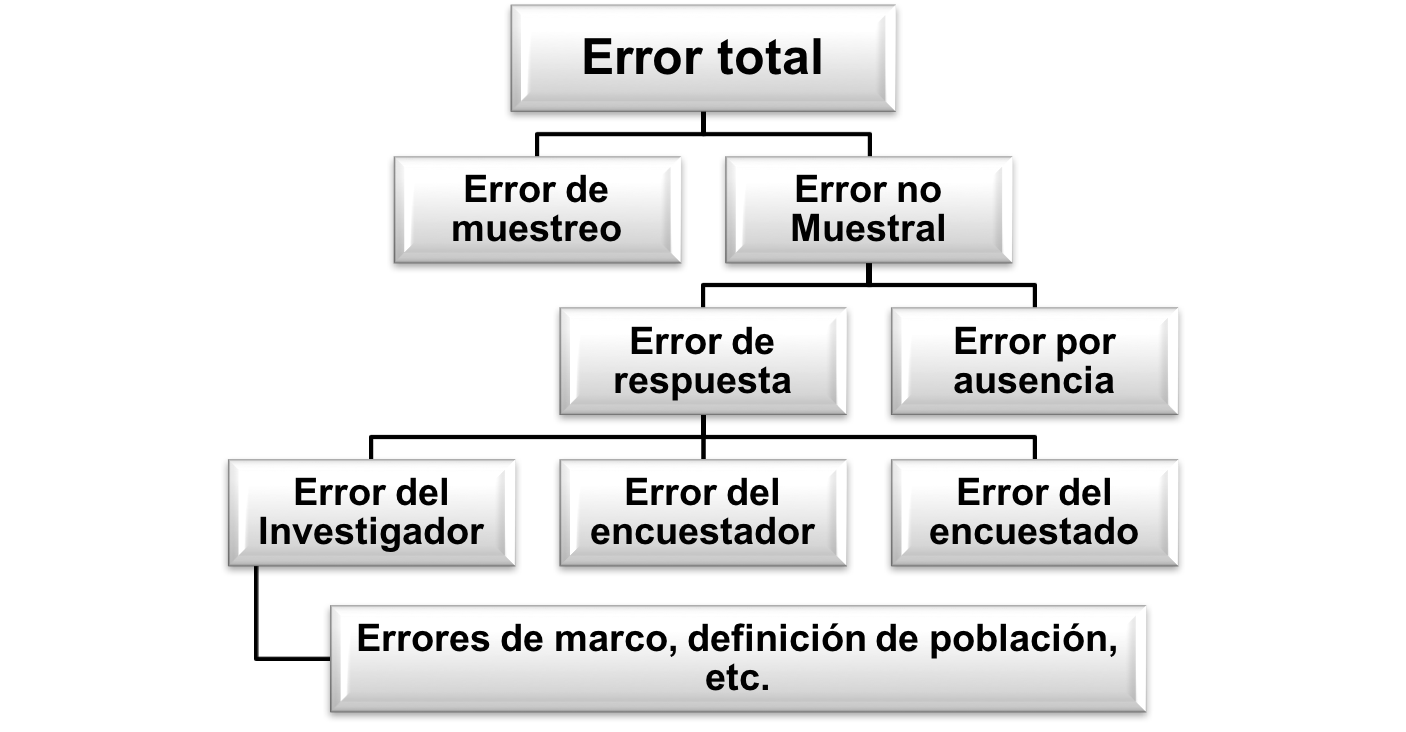
\includegraphics{Pics/Picture9.png}
\caption{\emph{El paradignma del error total. Fuente: adaptación de \citet{Groves_Fowler_Couper_Lepkowski_Singer_Tourangeau_2009}}}
\end{figure}

Por ejemplo, en una encuesta de fuerza laboral mensual, puede haber confusión en el respondiente si no se hace hincapíe en el periodo de referencia; no es lo mismo indagar por la semana pasada, que por el mes pasado y el respondiente debe ser guiado para evitar equivocaciones. Además pueden existir no respondientes en algún subgrupo de interés, o incluso el marco puede estar desactualizado. Uno de los objetivos de la planeación concienzuda de la encuesta es minimizar los errores no muestrales. Es necesario minimizar las discrepancias encontradas entre la respuesta verdadera a una pregunta y la respuesta final.

\citet{Groves_Fowler_Couper_Lepkowski_Singer_Tourangeau_2009} plantea que durante todo el siglo pasado, ha surgido una serie de teorías y principios que ofrecen un marco de referencia unificado en el diseño, implementación y evaluación de encuestas. Este marco de referencia se conoce comúnmente como el paradigma del error total de muestreo y ha encaminado la investigación moderna hacia una mejor calidad de las encuestas.

\hypertarget{sesgos-generados-en-las-encuestas}{%
\section{Sesgos generados en las encuestas}\label{sesgos-generados-en-las-encuestas}}

\citet{Gutierrez_2016} plantea que existen diferentes fuentes de sesgo en las encuestas y resume de la siguiente forma las dos fuentes de sesgo más importantes:

\hypertarget{sesgo-de-selecciuxf3n}{%
\subsection{Sesgo de selección}\label{sesgo-de-selecciuxf3n}}

Este tipo de sesgo ocurre cuando parte de la población objetivo no está en el marco de muestreo, o cuando el marco está incompleto y presenta deficiencias. Por ejemplo, una muestra a conveniencia\footnote{A pesar de que las muestras por conveniencia o por juicio no pueden ser utilizadas para estimar parámetros de la población, éstas sí pueden proporcionar información valiosa en las primeras etapas de una investigación o cuando no es necesario generalizar los resultados a la población.} es sesgada pues las unidades más fáciles de elegir o las que más probablemente respondan a la encuesta no son representativas de las unidades más difíciles de elegir. \citet{Loh} afirma que se presenta este tipo de sesgo si:

\begin{itemize}
\tightlist
\item
  La selección de la muestra depende de cierta característica asociada a las propiedades de interés. Por ejemplo: si la encuesta se realiza ingresando a un portal web, y precisamente las personas que no tienen cobertura de internet difieren significativamente de quienes sí tienen acceso.
\item
  La muestra se realiza mediante elección deliberada o mediante un juicio subjetivo. Por ejemplo, si el parámetro de interés es la cantidad promedio de gastos en compras en un centro comercial y el encuestador elige a las personas que salen con muchos paquetes, entonces la información estaría sesgada puesto que no está reflejando el comportamiento promedio de las compras.
\item
  Existen errores en la especificación de la población objetivo. Por ejemplo, en encuestas electorales, cuando la población objetivo contiene a personas que no están registradas como votantes ante la organización electoral de su país.
\item
  Existe sustitución deliberada de unidades no disponibles en la muestra. Si, por alguna razón, no fue posible obtener la medición y consecuente observación de la característica de interés para algún individuo en la población, la sustitución de este elemento debe hacerse bajo estrictos procedimientos estadísticos y no debe ser subjetiva en ningún modo.
\item
  Existe ausencia de respuesta. Este fenómeno puede causar distorsión de los resultados cuando los que no responden a la encuesta difieren críticamente de los que si respondieron.
\item
  La muestra está compuesta por respondientes voluntarios. Los foros radiales, las encuestas de televisión y los estudios de portales de internet no proporcionan información confiable.
\end{itemize}

Además de lo anterior, en América Latina pueden existir sesgos ocasionados por la falta de cobertura en el marco de muestreo, o por la exclusión planificada de subpoblaciones de difícil acceso. Por ejemplo, en una encuesta de fuerza de trabajo, es posible que la encuesta no sea representativa de las subpoblaciones afrodescendientes o indígenas, por no cubrir exhaustivamente los territorios donde se ubican.

\hypertarget{sesgo-de-mediciuxf3n}{%
\subsection{Sesgo de medición}\label{sesgo-de-mediciuxf3n}}

Este tipo de sesgo ocurre cuando el instrumento con el que se realiza la medición tiene una tendencia a diferir del valor verdadero que se desea averiguar. Este sesgo debe ser considerado y minimizado en la etapa de diseño de la encuesta. Si el instrumento de medición (cuestionario) tiene defectos en su planificación, entonces el resultado de la estimación en la encuesta seguramente diferirá sistemáticamente del verdadero valor para cada uno de los respondientes. Ningún análisis estadístico podrá ajustar esta diferencia sistemática. \citet{Loh} cita algunas situaciones en donde se presenta este sesgo de medición:

\begin{itemize}
\tightlist
\item
  Cuando el respondiente miente. Esta situación se presenta a menudo en encuestas que preguntan acerca del ingreso salarial, alcoholismo y drogadicción, nivel socioeconómico e incluso edad.
\item
  Cuando el cuestionario contiene preguntas difíciles de comprender. Por ejemplo: \emph{``¿No es cierto que usted no recibe remesas desde el exterior?''} La doble negación en esta pregunta es muy confusa para el respondiente.
\item
  Cuando hay un olvido del respondiente que no permite tener una respuesta veráz. Las personas tienden a olvidar, sobretodo las malas experiencias; esta situación debe acotarse si se está trabajando en una encuesta de criminalidad, victimización, consumo de sustancias psicoactivas, o módulos con preguntas sensibles.
\item
  Cuando se brindan distintas respuestas a diferentes entrevistadores. En algunas regiones es muy probable que la raza, edad o género del encuestador afecte directamente la respuesta del entrevistado.
\item
  Cuando se leen mal las preguntas o se polemiza con el respondiente. El encuestador puede influir notablemente en las respuestas. Por lo anterior, es muy importante que el proceso de entrenamiento del entrevistador sea riguroso y completo.
\item
  Cuando la muestra está compuesta por respondientes voluntarios. Los foros radiales, las encuestas de televisión y los estudios de portales de internet no proporcionan, en general, información confiable. En este caso también se presenta sesgo de selección.
\end{itemize}

\hypertarget{evoluciuxf3n-de-las-encuestas-estandarizadas}{%
\section{Evolución de las encuestas estandarizadas}\label{evoluciuxf3n-de-las-encuestas-estandarizadas}}

Cuando el mundo occidental superó los grandes traumatismos del siglo XX (dos guerras mundiales y una recesión a larga escala), la investigación social tuvo un auge sobresaliente a través de las encuestas por correo postal. Según lo comenta el \citet{INE2012}, en el caso Latinoamericano, la Agencia para el Desarrollo Internacional (AID) auspició la serie de catorce documentos ``Atlántida: Un Estudio de Caso en Encuesta de Hogares por Muestra'' (\citet{Atlantida}), elaborado por la Ofician de Censos los Estados Unidos de América, en el marco del Programa Alianza para el Progreso y presentado en colaboración con la Organización de Estados Americanos (OEA) y el Instituto Interamericano de Estadística. A partir de Atlántida se insituyó un modelo que serviría de apoyo para la realización de las encuestas de hogares en América Latina.

Desde el momento en que las encuestas de hogares se instauraron como un instrumento apropiado para la investigación, existen tres preguntas, en continua dinámica, que se deben responder para planificar, ejecutar y analizar una encuesta: ¿cómo se diseñarán las preguntas? ¿cómo se seleccionará la muestra? y ¿cómo se recolectarán las respuestas?

\hypertarget{inicio-de-los-cuestionarios-estandarizados}{%
\subsection{Inicio de los cuestionarios estandarizados}\label{inicio-de-los-cuestionarios-estandarizados}}

La práctica de realizar las mismas preguntas en forma de cuestionario es relativamente reciente. Antes de acoger un proceso estandarizado, cada encuestador podría preguntar ``lo mismo'', pero con diferentes palabras. Difícilmente, dos personas distintas eran entrevistadas con las mismas preguntas. \citet{Groves_Fowler_Couper_Lepkowski_Singer_Tourangeau_2009} mencionan que la forma en cómo se preguntaba y cómo se recopilaba la información afectaba dramáticamente los resultados de las encuestas. Fue así como se decidió que los encuestadores deberían ser entrenados formalmente.

Desde la psicometría se implementó el formalismo del cuestionario. Intentando medir estados psicológicos, afectivos e intelectuales, se desarrollaron técnicas apropiadas para hacer comparables las respuestas. \citet{Likert_1932} demostró que era posible realizar este tipo de comparaciones, evadiendo los largos instrumentos de medición, al formular una sola pregunta - a todos los encuestados - con una serie de respuestas en forma de escala.

\hypertarget{inicio-de-los-muxe9todos-de-muestreo}{%
\subsection{Inicio de los métodos de muestreo}\label{inicio-de-los-muxe9todos-de-muestreo}}

En un principio, los investigadores trataban de recolectar datos sobre todos los elementos de la población de interés. Esta práctica resultaba logísticamente inadecuada cuando se trataba de poblaciones con un gran tamaño. Los cálculos de los indicadores sobre toda una población resultaban muy demandantes. \citet{Groves_Fowler_Couper_Lepkowski_Singer_Tourangeau_2009} afirman que, aunque la teoría de la probabilidad tuvo sus orígenes en el siglo XVIII, no fue hasta la segunda década del siglo XX que se utilizó para realizar encuestas. La primera aplicación fue la selección sistemática de un elemento en una población enlistada. Para realizar esta selección, los registros censales se dividían en secciones y se procedía a seleccionar un elemento de la sección.

Más adelante, cuando la estadística permeó la agricultura, se definieron otros tipos de muestreo (menos demandantes) y se dio origen al muestreo de áreas. Es así como hoy en día es posible seleccionar muestras de bloques, zonas amanzanadas, secciones y sectores cartográficos, o áreas de empadronamiento censal. Se descubrió que era posible generalizar el muestreo de áreas y se creó el muestreo multietápico que permitió la selección de grandes bloques dentro de una ciudad, y áreas dentro de los bloques y el submuestreo sucesivo de unidades dentro hasta llegar a la unidad de interés. Todos estos submuestreos se realizan de forma probabilística.

La gran depresión en EE.UU. y la segunda guerra mundial fueron catalizadores de las encuestas a gran escala, puesto que en ese entonces, al igual que hoy, la tasa de desempleo era una cifra importante para la economía de los países. Por ende, las políticas públicas empezaron a decidirse de acuerdo con las estadísticas oficiales, puesto que las grandes encuestas empezaron a realizarse con una periodicidad mensual. Hoy en día existen cientos de encuestas mensuales que dan cuenta de la realidad de las sociedades en la región.

\hypertarget{inicio-de-la-recolecciuxf3n-de-datos}{%
\subsection{Inicio de la recolección de datos}\label{inicio-de-la-recolecciuxf3n-de-datos}}

Debido a que en un principio no existía un cuestionario estandarizado, entonces las respuestas abiertas eran la única opción de recopilar información. Esta práctica demandaba un gran esfuerzo en términos de resumir y sintetizar todo el corpus de palabras que los entrevistados usaban para responder.

En la mitad de la década del sesenta del siglo pasado, empezó una proliferación masiva de las entrevistas por correo en EE. UU. Los países con registros administrativos actualizados pueden contemplar este escenario puesto que induce altas tasas de cobertura a precios más económicos (pues se prescinde del encuestador). Las bajas tasas de respuestas (pues el encuestado debe llenar un formulario con sus respuestas y devolverlo a la oficina postal) hicieron que paulatinamente esta forma de recolección no fuese tan apetecida \citep{Groves_Fowler_Couper_Lepkowski_Singer_Tourangeau_2009}.

Como lo señala \citet{CEPALcuadernos}, en el caso latinoamericano en la primera parte del decenio de 1960 varios países de América Latina comenzaron a realizar encuestas de hogares periódicas con el propósito de obtener información sobre empleo y desempleo. En 1965 se realizó en la ciudad de México un seminario en que se presentó el estudio de Atlántida. Luego, ante la necesidad de satisfacer la demanda de información en relación con las políticas económicas y sociales, tomó gran impulso en varios países de la región la puesta en marcha de programas permanentes de encuestas de hogares dirigidos fundamentalmente a obtener información sobre la fuerza de trabajo. El modelo Atlántida se basó fundamentalmente en un modelo de encuesta empleado en países desarrollados que tienen mercado de trabajo con características propias. Sin embargo, resultó sumamente interesante para aquellos países que tenían poca experiencia en encuestas de hogares, y constituyó la base metodológica sobre la que se han establecido gran parte de las encuestas
de América Latina (\citet{CEPALcuadernos}).

Un camino intermedio entre la recolección de información presencial (cara a cara) y la recolección de información mediante formularios auto-administrados (por correo electrónico, mediante páginas de internet o mediante correo postal) son las entrevistas telefónicas. Hoy en día, la mayoría de sondeos en investigación de medios y de mercado se realiza por teléfono. Más aún, a partir de la pandemia por COVID-19, en marzo del 2020 el mundo sufrió una paralización de las actividades sociales y económicas, debido a los esfuerzos de los gobiernos para tratar de frenar la expansión de la pandemia en los países. Fue así como, debido a las restricciones de movilidad impuestas por los gobiernos, las operaciones estadísticas con levantamiento de datos presencial fueron suspendidas. En América Latina el rigor de la pandemia y de las medidas de restricción a la movilidad también afectaron el levantamiento de las encuestas de hogares. Sin embargo, a partir de estas dificultades \citet{CEPAL_continua} recomendó la continuidad de las encuestas mediante el uso de entrevistas telefónicas.

\hypertarget{el-ciclo-de-vida-de-una-encuesta}{%
\section{El ciclo de vida de una encuesta}\label{el-ciclo-de-vida-de-una-encuesta}}

Atendiendo al modelo de \citet{Groves_Fowler_Couper_Lepkowski_Singer_Tourangeau_2009}, se puede afirmar que en todas la encuestas se tienen dos niveles de inferencia: el individual y el grupal. El proceso de inferencia individual trata con los mismos respondientes que proveen la información primaria en el estudio; mientras que el el proceso de inferencia grupal, basado en una aproximación inductiva, va desde lo particular (la muestra) a lo general (la población).

\begin{figure}
\centering
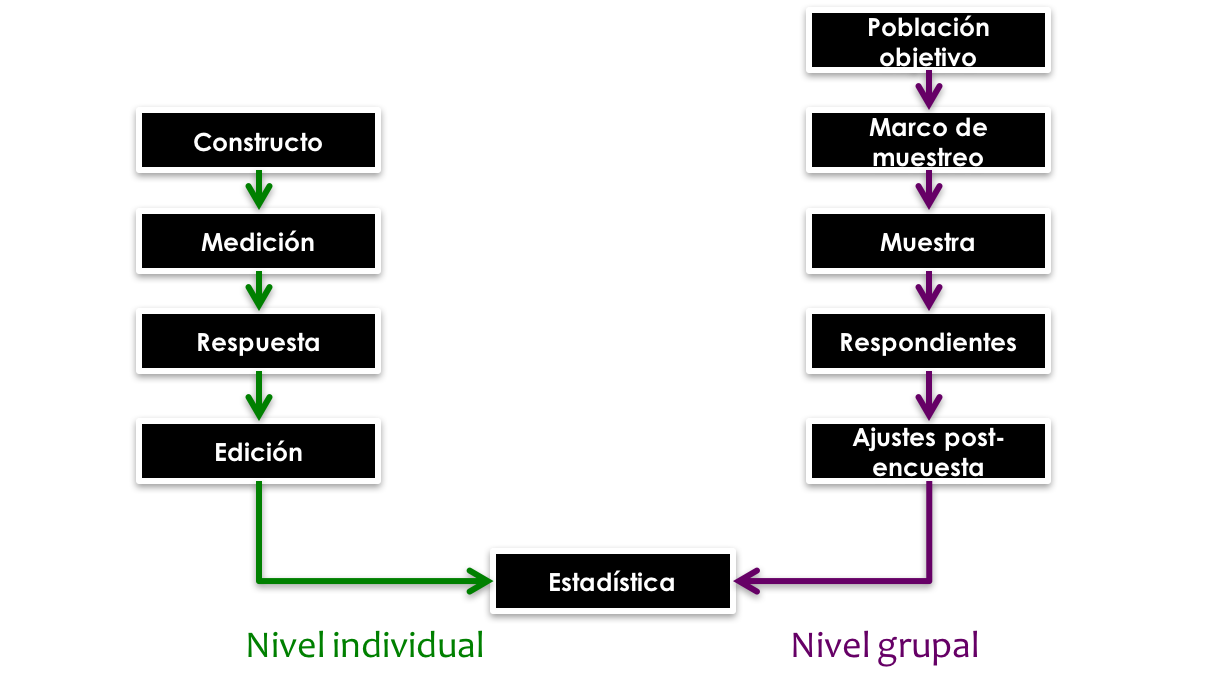
\includegraphics{Pics/Picture6.png}
\caption{\emph{Los niveles de inferencia en una encuestas. Fuente: adaptación de \citet{Groves_Fowler_Couper_Lepkowski_Singer_Tourangeau_2009}}}
\end{figure}

\hypertarget{inferencia-individual}{%
\subsection{Inferencia individual}\label{inferencia-individual}}

\hypertarget{constructo}{%
\subsubsection{Constructo}\label{constructo}}

\citet{Gutierrez_2016} menciona que los constructos son las ideas abstractas (ambiguas) sobre las cuales el investigador desea inferir y que, a su vez, dan origen a la investigación al ser la simiente de la encuesta. Las palabras con que se describen los constructos son siempre simples, pero la redacción elaborada de los constructos no siempre es precisa. Por ejemplo:

\begin{itemize}
\tightlist
\item
  En una \emph{encuesta de victimización} que mida la cantidad de incidentes relacionados con crímenes en un año determinado, es necesario definir muy apropiadamente qué se entiende por crimen, o cómo se define a una víctima, entre otros muchos aspectos.
\item
  En una \emph{encuesta de goce efectivo de derechos ciudadanos} sobre menores de edad se puede medir la efectividad del Estado al garantizar los derechos básicos a la primera infancia. Sin embargo, es necesario definir qué es un derecho, o cómo se define primera infancia.
\end{itemize}

Mientras que algunos constructos son más abstractos que otros (optimismo en la economía, confianza inversionista, percepción del Plan Nacional de Desarrollo de un gobierno), algunos otros son observables más concretamente (consumo de alcohol y otras drogas, nutrición en la primera infancia, productividad de una intervención en el sector agrícola, factores de riesgo asociados a una enfermedad).

\hypertarget{mediciones}{%
\subsubsection{Mediciones}\label{mediciones}}

La medición es una caracterización mucho más concreta que el constructo, puesto que representa una forma de obtener información de los constructos de interés. La cuestión clave para realizar una buena medición es realizar preguntas que induzcan respuestas que reflejen claramente los constructos que se desean medir. \citet{Groves_Fowler_Couper_Lepkowski_Singer_Tourangeau_2009} indican que estas preguntas pueden ser comunicadas en forma oral (encuestas cara a cara o telefónicas), o comunicadas en forma visual (atributos de un producto - marketing). Así mismo, también pueden existir observaciones directas del encuestador (condiciones de la vivienda), u observaciones provenientes de dispositivos electrónicos o físicos (precios de productos en supermercados, muestra de agua, muestra de sangre, etc.).

\hypertarget{respuesta-y-ediciuxf3n}{%
\subsubsection{Respuesta y edición}\label{respuesta-y-ediciuxf3n}}

El resultado de la medición es la respuesta y sus propiedades están determinadas por la naturaleza de las preguntas. Después de que los entrevistados han respondido, los datos deben pasar por un proceso de edición y validación de inconsistencias.

En este proceso de edición se debe examinar la distribución completa de las respuestas y buscar \emph{datos atípicos} para que sean revisados con detenimiento. Los datos editados constituyen el insumo para realizar todo el proceso de inferencia estadística pertinente para que las cifras resultantes sean confiables y precisas.

\hypertarget{inferencia-grupal}{%
\subsection{Inferencia grupal}\label{inferencia-grupal}}

\hypertarget{la-poblaciuxf3n-objetivo}{%
\subsubsection{La población objetivo}\label{la-poblaciuxf3n-objetivo}}

De las definiciones concernientes a agregados, esta es la más abstracta. En general, la \emph{población objetivo} representa el conjunto de unidades que serán estudiadas. Por ejemplo, en una encuesta es posible definir la población objetivo como los adultos nacionales. Sin embargo, esta definición de población no contempla el periodo de referencia de la medición, tampoco aclara si se incluyen los adultos residentes en el exterior y, no precisa cómo se verificará la nacionalidad de un entrevistado.

Por ende, la definición de la población objetiva tiene que ser lo más precisa posible. Por ejemplo, la Gran Encuesta Integrada de Hogares de Colombia define a su población objetivo como la Población civil no institucionalizada (PCNI), la cual contiene a todas las personas que no hacen parte de la fuerza pública y no pertenecen a instituciones de aislamiento como prisiones, hospitales, sanatorios, ancianatos, etc. La PCNI contiene a la población en edad de trabajar (PET) y a los no pertenecientes a la fuerza laboral. La edad para empezar a trabajar en el área rural es 10 años, y en la ciudad es 12 años. A su vez, la PET contiene a Inactivos y Ocupados. La clasificación de ocupado es una variable derivada que está inducida por muchos filtros.

\hypertarget{la-poblaciuxf3n-enmarcada}{%
\subsubsection{La población enmarcada}\label{la-poblaciuxf3n-enmarcada}}

No es posible realizar una encuesta probabilística sin un \emph{marco de muestreo}, definido como un dispositivo que permite ubicar e identificar (ambas acciones al mismo tiempo) las unidades pertenecientes a la población de interés. En América Latina, es a partir del censo que se construyen los marcos de muestreo para las encuestas de hogares en los países, miestras que en algunos países desarrollados es posible encontrar marcos de muestreo creados a partir de líneas telefónicas o dirección de residencia.

Es necesario darse cuenta de que todos los marcos de muestreo presentan algún nivel de desactualización con respecto a la población de interés. Por ejemplo, un marco de muestreo de áreas (basado en la cartografía del último ejercicio censa) puede estar desactualizado. Asimismo, algunas posibilidades negativas del uso de este tipo de marcos es que es posible entrevistar a la misma persona en varias ocasiones (si la persona tiene múltiples residencias), o incluso nunca realizar la entrevista a una persona que no tienen un lugar fijo de residencia. Por otra lado, un marco de muestreo de líneas telefónicas puede no contener a todos lo residentes de una ciudad.

La población enmarcada está definida por el conjunto de miembros de la población objetivo que efectivamente tienen una probabilidad no nula de ser seleccionados en una muestra probabilística. En general para definir quién pertenece a un hogar del marco existen dos alternativas:

\begin{enumerate}
\def\labelenumi{\arabic{enumi}.}
\tightlist
\item
  Regla \emph{de iure}: quien habitualmente reside en el hogar es miembro de ese hogar.

  \begin{itemize}
  \tightlist
  \item
    Una situación \emph{de iure} es aquella que está reconocida por la legalidad vigente o por la autoridad competente en virtud de algún acuerdo o acto formal.
  \item
    Evita la subcobertura de individuos que no residen usualmente en su hogar, considerándolo suyo.
  \end{itemize}
\item
  Regla \emph{de facto}: quien pasó la noche anterior en una residencia de un hogar es miembro de ese hogar.

  \begin{itemize}
  \tightlist
  \item
    Una situación \emph{de facto} es aquella que, existiendo en la realidad, no ha sido reconocida formalmente.
  \item
    Evita la sobrecobertura de individuos que tienen más de una residencia.
  \end{itemize}
\end{enumerate}

\hypertarget{la-muestra}{%
\subsubsection{La muestra}\label{la-muestra}}

El tamaño de muestra define directamente la precisión y confiabilidad de las estimaciones. Este debería incrementarse a medida que lo hagan los niveles de desagregación (grupos etarios, regiones geográficas, niveles de escolaridad, etc.). Sin embargo, dependiendo de la caracterización de la estrategia de muestreo, pueden existir escenarios en donde una encuesta con un tamaño de muestra menor induzca menores errores de muestreo que una encuesta con un mayor tamaño de muestra.

No obstante, en algunas ocasiones los esfuerzos realizados para que los individuos seleccionados en la muestra respondan no son fructíferos. De esta manera, los individuos que son efectivamente entrevistados se denominan respondientes efectivos; mientras que al complemento de este conjunto se les denomina no respondientes.

\hypertarget{los-respondientes}{%
\subsubsection{Los respondientes}\label{los-respondientes}}

Pueden existir casos de no respondientes parciales (no respondientes de ítems), para los cuales debe existir un proceso de \emph{decisión} en términos de su reemplazo. Asimismo, no todas las ausencias parciales son reemplazadas. \citet{Groves_Fowler_Couper_Lepkowski_Singer_Tourangeau_2009} afirman que algunos de los factores que inciden en el aumento de la ausencia de respuesta pueden ser causados por:

\begin{itemize}
\tightlist
\item
  \emph{Contenido}: por preguntas sensibles (encuestas relacionadas con el uso de drogas, finanzas, victimización). En este caso, se puede acotar la tasa de respuesta si se ordenan las preguntas de manera adecuada.
\item
  \emph{Encuestadores}: aplicar métodos estándar de mejoramiento de la calidad para aumentar la precisión y tasa de respuesta de los entrevistadores involucrados en el estudio.
\item
  \emph{Método de recolección}: las encuestas telefónicas, por correo electrónico o por páginas web tienen una tasa de respuesta menor que las entrevistas personales.
\item
  \emph{Diseño de cuestionario}: mala planificación en el pase de las preguntas que conforman el instrumento.
\item
  \emph{Tiempo de la encuesta y agobio}: algunas temporadas arrojan tasas de no respuestas más altas que otras. De la misma forma, algunos cuestionarios largos son propensos a inducir una mayor ausencia de respuesta parcial por el agotamiento del respondiente. En general, las encuestas demasiado largas pueden indisponer al respondiente.
\end{itemize}

\hypertarget{los-ajustes-post-encuesta}{%
\subsubsection{Los ajustes post-encuesta}\label{los-ajustes-post-encuesta}}

Toda encuesta cuenta con personas que no quisieron responder y/o con un marco de muestreo que no cubre a toda la población. Por ende, es necesario realizar algunos ajustes en el análisis y procesamiento para evitar, sobretodo, la sub-estimación de los parámetros de interés, o implementar métodos de imputación para suplir la información faltante. De esta forma se puede utilizar una reponderación diferencial cuando es evidente que hay un patrón de ausencia de respuesta en algunos subgrupos de la población; por ejemplo: si las tasas de respuestas a nivel urbano son menores que las tasas de respuesta a nivel rural, o si los hombres responden menos que las mujeres.

También es posible imputar (cuya raíz inglesa es \emph{input}, traducido como introducir valores) los valores perdidos en un subconjunto de observaciones de la muestra seleccionada. En este caso es factible utilizar metodologías estocásticas complejas para imputar valores, o técnicas simples sistemáticas. Sin embargo, en cualquier caso, siempre es preferible obtener la respuesta directa del entrevistado.

\hypertarget{el-proceso-de-respuesta}{%
\section{El proceso de respuesta}\label{el-proceso-de-respuesta}}

No todas las encuestas se planean de tal forma que exista una interacción directa entre respondiente y entrevistador en todo tiempo. Sin emabrgo los modelo de respuesta en las encuestas asumen que existen, por lo menos, lo siguientes momentos en la obtención de un valor numérico que se recopila como respuesta al cuestionario:

\begin{enumerate}
\def\labelenumi{\arabic{enumi}.}
\tightlist
\item
  \emph{La comprensión}, momento en donde el respondiente interpreta la pregunta. \citet{Groves_Fowler_Couper_Lepkowski_Singer_Tourangeau_2009} afirman que en este momento se involucran todos aquellos procesos de atención a la pregunta y entendimiento de las instrucciones. La primera tarea del respondiente es interpretar la pregunta y, al hacerlo surgen procesos de análisis y asignación de un significado a los elementos sustantivos de la pregunta. Además el respondiente debe hacer una inferencia sobre el propósito de la pregunta, determinar los límites de la respuesta, así como acotar los posibles traslapes sobre las respuestas permitidas.
\item
  \emph{El recaudo}, momento en donde el respondiente recolecta en su memoria la información necesaria para brindar una respuesta. En algunas ocasiones se accede a la memoria de largo plazo que almacena todo el contenido autobiográfico y el conocimiento general. Nótese que muchas cosas pueden afectar el desempeño de la memoria de largo plazo (cuando los eventos en cuestión no se distinguen con facilidad o cuando los eventos no tienen un gran impacto personal). La memoria provee la información relevante para que el entrevistado proporcione una respuesta adecuada. Este ciclo de recaudo de información continúa hasta que el entrevistado dé una respuesta acertada o simplemente no quiera recordar más (algunas situaciones son más difíciles de recordar) \citep{Groves_Fowler_Couper_Lepkowski_Singer_Tourangeau_2009}. Para ayudar a la memoria de largo plazo se pueden diseñar señales o pistas auto-contenidas en la pregunta. Las mejores señales son las que ofrecen un nivel de detalle más profundo.
\item
  \emph{El juicio}, momento en donde se combina, se pondera y se resume la información recolectada. En esta etapa se surten procesos que complementan los recaudos que el entrevistado ha contemplado anteriormente. El juicio puede llenar los vacíos de la memoria, combinar los recaudos o ajustarlos por omisión. Por ejemplo, en una encuesta de ingresos y gastos, las personas, por lo general, no llevan la cuenta del número de veces que compraron cierto artículo o no tienen una respuesta predefinida al número de veces que han salido de compras. Por ende, el respondiente tratará de contar el número de veces que experimentó una situación, y si ese número es muy grande, seguramente se acercará a la respuesta mediante una estimación. La estrategia de estimación del respondiente (llevar la cuenta, construir una escala mediante la recordación de eventos, realizar una estimación gruesa o adivinar al azar) depende del número de sucesos, su duración, la regularidad de los mismos y el periodo de referencia de la encuesta \citep{Groves_Fowler_Couper_Lepkowski_Singer_Tourangeau_2009}.
\item
  \emph{El reporte}, momento en donde el respondiente formula su respuesta y la estandariza en el formato inducido por el cuestionario. Este es el proceso de selección y comunicación de una respuesta, que incluye el encuadre de la respuesta dentro de las opciones que provee la pregunta (también implica alterar la respuesta para que se ajuste a las opciones aceptables). La forma en que se reporta la respuesta final dependerá del ajuste que se realice en los procesos de recaudo y estimación y las restricciones que la pregunta impone. En este sentido, si para una pregunta de percepción la mayoría de opciones de respuesta son negativas, la respuesta estará sesgada en esa dirección. Asimismo, los respondientes pueden dar mayor importancia a ciertas opciones de respuesta \citep{Groves_Fowler_Couper_Lepkowski_Singer_Tourangeau_2009}.
\end{enumerate}

El investigador debe saber que el solo hecho de haber experimentado una situación, no implica que el respondiente haya compilado la suficiente información para reportarla como respuesta. \citet{Groves_Fowler_Couper_Lepkowski_Singer_Tourangeau_2009} afirman que se ha visto que los testigos presenciales de una situación omiten detalles importantes acerca de la situación de la cual son testigos. Además, las personas no pueden proveer la información que no tienen. Si la gente no compila la información necesaria, ninguna pregunta ni formulación logrará obtener la respuesta real. Por lo que se recomienda llevar a cabo las pruebas necesarias para validar el cuestionario. Por otro lado, aunque el respondiente conozca con exactitud la respuesta a una pregunta, no será capaz de reportarla correctamente si no hay una buena interpretación de la misma.

Por otra parte, es necesario advertir que la respuesta del entrevistado también está supeditada a los tiempos de ocurrencia (los eventos que sucedieron hace mucho tiempo son más difíciles de recordar), a los límites temporales y su correspondiente impacto emocional, puesto que los eventos cercanos a momentos que generan impacto emocional son más fáciles de recordar (eventos catastróficos, atentados terroristas o desastres naturales) y también a las señales en las preguntas, pues la asignación de múltiples señales en la redacción de la pregunta ayuda a activar el proceso de recordación.

En cuanto a la naturaleza de las preguntas, se puede notar que las preguntas cerradas con escala ordenada podrían tender a producir un sesgo de respuesta positivo, pues los respondientes tienden a evadir las opciones negativas de la escala (encuestas de satisfacción). \citet{Schwarz1991} demostró que las etiquetas numéricas afectan el proceso de respuesta, por lo cual recomendó que el encuestador no lea los números en las opciones de respuesta, así como acotar el número de opciones en preguntas de opinión (no muy pocas, no tantas).

Así mismo, nótese que la generación de pocas opciones de respuesta hace que se pierda el poder de discriminación, mientras que utilizar muchas opciones puede hacer que los encuestados no distingan fácilmente entre las categorías adyacentes. Además, es posible que el respondiente no quiera esperar a que el entrevistador lea exhaustivamente todas las opciones de respuesta. En este caso se presentan dos fenómeno que es necesario evadir. En primer lugar el efecto de primacía, el cual incrementa el riesgo de que el respondiente escoja una de las primeras opciones; y el efecto de recencia, en donde el respondiente siempre escogerá una de las últimas opciones.

Algunos respondientes podrán desviarse del modelo de respuesta mediante la escogencia de rutas alternas de evasión (el encuestado hará el mínimo esfuerzo para satisfacer las demandas del entrevistador). Es así como podríamos encontrar respondientes que seleccionan sistemáticamente las opciones \emph{No sabe} o \emph{No responde}, o que escogen siempre la misma opción para cada pregunta. Inclusive, dependiendo de la apariencia del entrevistador, el respondiente puede estar sesgado a siempre estar de acuerdo (aquiescencia). De la misma manera, es posible que el respondiente quiera presentarse a sí mismo de manera favorable, omitiendo sus atributos no deseables \citep{Groves_Fowler_Couper_Lepkowski_Singer_Tourangeau_2009}.

\hypertarget{elementos-estaduxedsticos-buxe1sicos-en-la-planeaciuxf3n-de-las-encuestas}{%
\chapter{Elementos estadísticos básicos en la planeación de las encuestas}\label{elementos-estaduxedsticos-buxe1sicos-en-la-planeaciuxf3n-de-las-encuestas}}

El fortalecimiento continuo de las investigaciones sociales es un objetivo que los institutos nacionales de estadística procuran cumplir de forma sistemática. En el caso de aquellas operaciones que conllevan la recolección de información primaria y que involucran la selección y medición de hogares y sus miembros, mantener una documentación adecuada que describa las razones por las cuales se ha optado por cierta metodología de recolección en particular es un requisito fundamental para cumplir este cometido. En este apartado se exploran diferentes métodos de recolección de la información y se discuten las diferentes particularidades en la planeación de una encuesta de hogares.

\hypertarget{universo-muestra-y-unidades}{%
\section{Universo, muestra y unidades}\label{universo-muestra-y-unidades}}

El término encuesta se encuentra directamente relacionado con una población finita compuesta de individuos a los cuales es necesario observar y medir. Este proceso es realizado por medio de una entrevista presencial, telefónica o mediante formularios electrónicos autoadministrados. El conjunto de unidades de interés recibe el nombre de \emph{población objetivo} o \emph{universo} y sobre ellas se obtiene la información de interés para el estudio. Por ejemplo, \emph{la Encuesta Nacional de Empleo y Desempleo} de Ecuador define su población objetivo como todas las personas mayores de 10 años residentes en viviendas particulares en Ecuador \citep{INEC-EC}.

Las \emph{unidades de análisis} corresponden a los diferentes niveles de desagregación establecidos para consolidar el diseño de la encuesta y sobre los que se presentan los resultados de interés. En México, la \emph{Encuesta Nacional de Ingresos y Gastos de los Hogares} define como unidades de análisis el ámbito al que pertenece la vivienda: urbano alto, complemento urbano y rural. Por otro lado, la \emph{Gran Encuesta Integrada de Hogares} de Colombia tiene cobertura nacional y sus unidades de análisis están definidas por trece grandes ciudades junto con sus áreas metropolitanas \citep{DANE-COL_2017}.

Como se explicará más adelante, es muy difícil contar con una lista actualizada de todos los hogares del país; por lo tanto, para recolectar la información de la población objetivo, el diseño de una encuesta de hogares en América Latina plantea la necesidad de seleccionar en varias etapas ciertas \emph{unidades de muestreo} que sirven como medio para seleccionar finalmente a los hogares y personas que participarán de la muestra. Cuando se requiere seleccionar personas, se hace necesario seleccionar un subconjunto de zonas geográficas; para cada zona seleccionada, se procede a seleccionar a su vez un subconjunto de secciones cartográficas, que antecede a la selección de hogares. Finalmente, el cuestionario es administrado en cada hogar a un respondiente idóneo, que proporciona la información de todos los integrantes del hogar. Dependiendo de la encuesta, en algunos casos se seleccionan aleatoriamente respondientes individuales dentro del hogar; siendo estas las unidades de observación. Por ejemplo, se puede citar la experiencia de Brasil con la \emph{Pesquisa Nacional por Amostra de Domicilios} que se realiza por medio de una muestra de viviendas en tres etapas: las unidades primarias de muestreo (UPM) son los municipios, mientras que las unidades secundarias de muestreo (USM) son los sectores censales, que conforman una malla territorial definida en el último \emph{Censo Demográfico}. Por último, las unidades finales en ser seleccionadas son las viviendas \citep{IBGE_2014}.

\citet[pág. 105]{Duncan_Kalton_1987} afirman que la composición de la población de interés en las encuestas de hogares cambia durante el tiempo, puesto que lo individuos nacen, mueren, migran, e incluso pasan a ser parte de organizaciones que hacen que pierdan su estatus de elegibilidad como unidades de observación en una encuesta. Nótese que la población objetivo de la mayoría de encuestas de hogares en América Latina se refiere a la población civil excluyendo a los miembros de organizaciones militares, personas recluidas en cárceles, personas que se encuentran en hospitales, etc. De igual forma, se debe tener en cuenta que los hogares pueden crearse o desintegrarse rápidamente. Por ende, los equipos técnicos de las ONE que están a cargo del diseño de las encuestas de hogares, que miden de forma transversal a la población de interés, deben tener en cuenta que, aunque los objetivos de la encuesta no cambian en el tiempo, sí lo hace la población objetivo y se deben plantear esquemas de seguimiento y actualización que den cuenta de esta realidad.

\hypertarget{periodicidad-en-el-tiempo}{%
\section{Periodicidad en el tiempo}\label{periodicidad-en-el-tiempo}}

Las Oficinas Nacionales de Estadística - que son los entes encargados de administrar, diseñar, analizar y difundir los resultados de las encuestas - no realizan este tipo de levantamientos de manera aislada; de hecho una característica fundamental de estas operaciones estadísticas es que se han convertido en un insumo fundamental para realizar un seguimiento periódico de muchos indicadores de interés. Por lo tanto, muchas encuestas de hogares se realizan de forma sistemática en el tiempo, aunque algunas otras no tienen una periodicidad predefinida. Es por esto que la planeación de la encuesta debe contemplar este tipo de esquemas continuos para que el levantamiento de la información primaria en campo se haga de manera más eficiente y, de la misma forma, que la estimación de los indicadores de interés se pueda realizar ajustándose a los recursos de la operación. Como se mencionó anteriormente, dado que la población es dinámica en el tiempo, la planeación y análisis de este tipo de encuestas es desafiante, puesto que si la composición de la población y las características de los elementos se considerara fija, una encuesta transversal (realizada una sola vez en un periodo de tiempo largo) sería suficiente para realizar estimaciones precisas que resuelvan los objetivos del estudio.

En algunas ocasiones, basta con realizar un medición simple en un punto específico del tiempo para completar los objetivos de la investigación. Este es el caso de las encuestas de ingresos y gastos cuya periodicidad es, en general, no menor a cinco años y las cuales son utilizadas para, entre muchos otros propósitos, actualizar la canasta básica familiar, de la cual se derivan los insumos básicos para la medición de la pobreza \citep{CEPAL_2018}. Para otro tipo de problemáticas, como por ejemplo el seguimiento a las estadísticas derivadas del mercado de trabajo, es necesario recurrir a la medición periódica a través de encuestas de hogares, en donde los cambios naturales en las características de la población hacen que realizar una medición simple en un punto del tiempo sea insuficiente a la luz del seguimiento y monitoreo de los indicadores de interés.

Por consiguiente, al momento de realizar la planeación de una encuesta continua o periódica se debe tener en cuenta que, a pesar de que crezca la dificultad en el diseño, es posible obtener información más oportuna para la toma de decisiones y la formulación de políticas públicas. De esta manera, y teniendo en cuenta que el tiempo hace que la estructura de las poblaciones cambie, sin importar si la constituyen individuos, hogares, familias, negocios, etc., las unidades de observación deben ser consideradas como parte de la población de interés cuando nacen, inmigran o alcanzan un umbral predefinido de edad. Asimismo, las unidades ya no harán parte de la población de interés cuando mueran, emigren, o se involucren en instituciones (como el servicio militar). Por ejemplo, si las unidades de interés son los hogares, es evidente que la población no es la misma en diferentes puntos del tiempo (por ejemplo, en dos años distintos) puesto que se crean nuevas unidades cuando los jóvenes dejan a sus padres y forman nuevos hogares independientes, o cuando ocurre una separación o un divorcio; en donde un hogar se divide en dos. Además, los hogares en donde todos sus miembros han fallecido dejan de ser parte de la población objetivo. De la misma forma, dos hogares dejan de ser parte de la población objetivo cuando se unen a través de un matrimonio o algún otro tipo de unión civil, formando un nuevo hogar.

Teniendo en cuenta el papel dinámico de las poblaciones y los objetivos de investigación es posible plantear diferentes tipos de levantamientos; a continuación enumeramos algunas categorías de encuestas que las ONE realizan en la región.

\hypertarget{encuestas-transversales}{%
\subsection{Encuestas transversales}\label{encuestas-transversales}}

Este tipo de encuestas son diseñadas para recolectar información únicamente en un punto específico del tiempo, o sobre un periodo de referencia, y proveen toda la información pertinente acerca de la población particular restringida a un tiempo y periodo de recolección específico. Puesto que el propósito fundamental de este tipo de encuestas no se centra en las comparaciones intertemporales, no es posible estimar cambios de ningún tipo, a no ser que se realicen indagaciones retrospectivas. La siguiente tabla muestra un esquema de este tipo de operaciones estadísticas en donde se observa una muestra de una población específica en un periodo de tiempo específico (Tiempo 2). Dado que es una muestra transversal, no hay un patrón de repetición en los restantes periodos.

\begin{longtable}[]{@{}
  >{\centering\arraybackslash}p{(\columnwidth - 12\tabcolsep) * \real{0.1304}}
  >{\centering\arraybackslash}p{(\columnwidth - 12\tabcolsep) * \real{0.1449}}
  >{\centering\arraybackslash}p{(\columnwidth - 12\tabcolsep) * \real{0.1449}}
  >{\centering\arraybackslash}p{(\columnwidth - 12\tabcolsep) * \real{0.1449}}
  >{\centering\arraybackslash}p{(\columnwidth - 12\tabcolsep) * \real{0.1449}}
  >{\centering\arraybackslash}p{(\columnwidth - 12\tabcolsep) * \real{0.1449}}
  >{\centering\arraybackslash}p{(\columnwidth - 12\tabcolsep) * \real{0.1449}}@{}}
\caption{\emph{Esquema de una encuesta transversal.}}\tabularnewline
\toprule()
\begin{minipage}[b]{\linewidth}\centering
Hogar
\end{minipage} & \begin{minipage}[b]{\linewidth}\centering
Tiempo 1
\end{minipage} & \begin{minipage}[b]{\linewidth}\centering
Tiempo 2
\end{minipage} & \begin{minipage}[b]{\linewidth}\centering
Tiempo 3
\end{minipage} & \begin{minipage}[b]{\linewidth}\centering
Tiempo 4
\end{minipage} & \begin{minipage}[b]{\linewidth}\centering
\ldots{}
\end{minipage} & \begin{minipage}[b]{\linewidth}\centering
Tiempo \(T\)
\end{minipage} \\
\midrule()
\endfirsthead
\toprule()
\begin{minipage}[b]{\linewidth}\centering
Hogar
\end{minipage} & \begin{minipage}[b]{\linewidth}\centering
Tiempo 1
\end{minipage} & \begin{minipage}[b]{\linewidth}\centering
Tiempo 2
\end{minipage} & \begin{minipage}[b]{\linewidth}\centering
Tiempo 3
\end{minipage} & \begin{minipage}[b]{\linewidth}\centering
Tiempo 4
\end{minipage} & \begin{minipage}[b]{\linewidth}\centering
\ldots{}
\end{minipage} & \begin{minipage}[b]{\linewidth}\centering
Tiempo \(T\)
\end{minipage} \\
\midrule()
\endhead
1 & & \textbf{x} & & & & \\
2 & & \textbf{x} & & & & \\
3 & & \textbf{x} & & & & \\
4 & & \textbf{x} & & & & \\
\ldots{} & & \textbf{x} & & & & \\
\(n\) & & \textbf{x} & & & & \\
\bottomrule()
\end{longtable}

\hypertarget{encuestas-repetidas}{%
\subsection{Encuestas repetidas}\label{encuestas-repetidas}}

Cuando existe interés en realizar un seguimiento del fenómeno en observación durante el tiempo, se utilizan encuestas repetidas que recolectan información de manera periódica. Este tipo de encuestas proveen información acerca de la dinámica de la composición de la población en el tiempo. De esta forma, en cada levantamiento se observa una muestra de la población en un tiempo determinado. Por ejemplo, la siguiente tabla muestra un acercamiento gráfico a este tipo de encuestas en donde se evidencia el carácter sistemático de estas operaciones estadísticas; además de mostrar que no es posible medir cambios individuales porque las muestras son independientes en el tiempo.

\begin{longtable}[]{@{}
  >{\centering\arraybackslash}p{(\columnwidth - 12\tabcolsep) * \real{0.1304}}
  >{\centering\arraybackslash}p{(\columnwidth - 12\tabcolsep) * \real{0.1449}}
  >{\centering\arraybackslash}p{(\columnwidth - 12\tabcolsep) * \real{0.1449}}
  >{\centering\arraybackslash}p{(\columnwidth - 12\tabcolsep) * \real{0.1449}}
  >{\centering\arraybackslash}p{(\columnwidth - 12\tabcolsep) * \real{0.1449}}
  >{\centering\arraybackslash}p{(\columnwidth - 12\tabcolsep) * \real{0.1449}}
  >{\centering\arraybackslash}p{(\columnwidth - 12\tabcolsep) * \real{0.1449}}@{}}
\caption{\emph{Esquema de una encuesta repetida.}}\tabularnewline
\toprule()
\begin{minipage}[b]{\linewidth}\centering
Hogar
\end{minipage} & \begin{minipage}[b]{\linewidth}\centering
Tiempo 1
\end{minipage} & \begin{minipage}[b]{\linewidth}\centering
Tiempo 2
\end{minipage} & \begin{minipage}[b]{\linewidth}\centering
Tiempo 3
\end{minipage} & \begin{minipage}[b]{\linewidth}\centering
Tiempo 4
\end{minipage} & \begin{minipage}[b]{\linewidth}\centering
\ldots{}
\end{minipage} & \begin{minipage}[b]{\linewidth}\centering
Tiempo \(T\)
\end{minipage} \\
\midrule()
\endfirsthead
\toprule()
\begin{minipage}[b]{\linewidth}\centering
Hogar
\end{minipage} & \begin{minipage}[b]{\linewidth}\centering
Tiempo 1
\end{minipage} & \begin{minipage}[b]{\linewidth}\centering
Tiempo 2
\end{minipage} & \begin{minipage}[b]{\linewidth}\centering
Tiempo 3
\end{minipage} & \begin{minipage}[b]{\linewidth}\centering
Tiempo 4
\end{minipage} & \begin{minipage}[b]{\linewidth}\centering
\ldots{}
\end{minipage} & \begin{minipage}[b]{\linewidth}\centering
Tiempo \(T\)
\end{minipage} \\
\midrule()
\endhead
1 & \textbf{x} & & & & & \\
2 & & \textbf{x} & & & & \\
3 & & & \textbf{x} & & & \\
4 & & & & \textbf{x} & & \\
\ldots{} & & & & & \textbf{x} & \\
\(n\) & & & & & & \textbf{x} \\
\bottomrule()
\end{longtable}

\hypertarget{encuestas-panel}{%
\subsection{Encuestas panel}\label{encuestas-panel}}

Las encuestas en panel están diseñadas para recolectar información periódica sobre la misma muestra en diferentes puntos del tiempo. Por definición, las unidades de muestreo son las mismas en los diferentes periodos de tiempo y, de manera general, se miden las mismas variables en cada levantamiento. Por la caracterización propia de este tipo de encuestas, sí es posible estimar los cambios individuales, así como los cambios netos sobre la población. Sin embargo, como la muestra no cambia en ningún momento del tiempo, las inferencias que se realicen estarán supeditadas a la población de la cual se seleccionó la muestra en un principio (Tiempo 1). Si la población cambia su estructura, no será posible captar este cambio puesto que las inferencias resultantes de este tipo de encuestas no son representativas de la población actual. La siguiente tabla muestra un esquema propio de las encuestas de panel en donde los individuos que fueron seleccionados la primera vez son observados a lo largo del tiempo.

\begin{longtable}[]{@{}
  >{\centering\arraybackslash}p{(\columnwidth - 12\tabcolsep) * \real{0.1304}}
  >{\centering\arraybackslash}p{(\columnwidth - 12\tabcolsep) * \real{0.1449}}
  >{\centering\arraybackslash}p{(\columnwidth - 12\tabcolsep) * \real{0.1449}}
  >{\centering\arraybackslash}p{(\columnwidth - 12\tabcolsep) * \real{0.1449}}
  >{\centering\arraybackslash}p{(\columnwidth - 12\tabcolsep) * \real{0.1449}}
  >{\centering\arraybackslash}p{(\columnwidth - 12\tabcolsep) * \real{0.1449}}
  >{\centering\arraybackslash}p{(\columnwidth - 12\tabcolsep) * \real{0.1449}}@{}}
\caption{\emph{Esquema de una encuesta tipo panel.}}\tabularnewline
\toprule()
\begin{minipage}[b]{\linewidth}\centering
Hogar
\end{minipage} & \begin{minipage}[b]{\linewidth}\centering
Tiempo 1
\end{minipage} & \begin{minipage}[b]{\linewidth}\centering
Tiempo 2
\end{minipage} & \begin{minipage}[b]{\linewidth}\centering
Tiempo 3
\end{minipage} & \begin{minipage}[b]{\linewidth}\centering
Tiempo 4
\end{minipage} & \begin{minipage}[b]{\linewidth}\centering
\ldots{}
\end{minipage} & \begin{minipage}[b]{\linewidth}\centering
Tiempo \(T\)
\end{minipage} \\
\midrule()
\endfirsthead
\toprule()
\begin{minipage}[b]{\linewidth}\centering
Hogar
\end{minipage} & \begin{minipage}[b]{\linewidth}\centering
Tiempo 1
\end{minipage} & \begin{minipage}[b]{\linewidth}\centering
Tiempo 2
\end{minipage} & \begin{minipage}[b]{\linewidth}\centering
Tiempo 3
\end{minipage} & \begin{minipage}[b]{\linewidth}\centering
Tiempo 4
\end{minipage} & \begin{minipage}[b]{\linewidth}\centering
\ldots{}
\end{minipage} & \begin{minipage}[b]{\linewidth}\centering
Tiempo \(T\)
\end{minipage} \\
\midrule()
\endhead
1 & \textbf{x} & \textbf{x} & \textbf{x} & \textbf{x} & \textbf{x} & \textbf{x} \\
2 & \textbf{x} & \textbf{x} & \textbf{x} & \textbf{x} & \textbf{x} & \textbf{x} \\
3 & \textbf{x} & \textbf{x} & \textbf{x} & \textbf{x} & \textbf{x} & \textbf{x} \\
4 & & & & & & \\
\ldots{} & & & & & & \\
\(n\) & & & & & & \\
\bottomrule()
\end{longtable}

\hypertarget{encuestas-de-panel-dividido}{%
\subsection{Encuestas de panel dividido}\label{encuestas-de-panel-dividido}}

Para hacerle frente a las dificultades propias de las encuestas de panel y poder observar tanto los cambios individuales, como los cambios en la estructura de la población, se definen las encuestas de panel dividido. Estas operaciones estadísticas son una combinación del diseño de panel puro y del diseño repetido y su objetivo es realizar inferencias precisas acerca de los cambios de una cohorte a través del tiempo y, al mismo tiempo, del cambio en estructura de la población actual. De esta forma, se realiza el seguimiento continuo, periódico y sistemático de una muestra a través del tiempo, pero en cada levantamiento se incluyen nuevos elementos seleccionados de la población actual. Como se señalará más adelante, este tipo de encuestas cubre con eficiencia la mayoría de indicadores de interés en un estudio de investigación social. La siguiente tabla muestra una caracterización de estos levantamientos que fijan una muestra de panel a lo largo del tiempo, y a la vez que se añaden nuevas observaciones.

\begin{longtable}[]{@{}
  >{\centering\arraybackslash}p{(\columnwidth - 12\tabcolsep) * \real{0.1304}}
  >{\centering\arraybackslash}p{(\columnwidth - 12\tabcolsep) * \real{0.1449}}
  >{\centering\arraybackslash}p{(\columnwidth - 12\tabcolsep) * \real{0.1449}}
  >{\centering\arraybackslash}p{(\columnwidth - 12\tabcolsep) * \real{0.1449}}
  >{\centering\arraybackslash}p{(\columnwidth - 12\tabcolsep) * \real{0.1449}}
  >{\centering\arraybackslash}p{(\columnwidth - 12\tabcolsep) * \real{0.1449}}
  >{\centering\arraybackslash}p{(\columnwidth - 12\tabcolsep) * \real{0.1449}}@{}}
\caption{\emph{Esquema de una encuesta de panel dividido.}}\tabularnewline
\toprule()
\begin{minipage}[b]{\linewidth}\centering
Hogar
\end{minipage} & \begin{minipage}[b]{\linewidth}\centering
Tiempo 1
\end{minipage} & \begin{minipage}[b]{\linewidth}\centering
Tiempo 2
\end{minipage} & \begin{minipage}[b]{\linewidth}\centering
Tiempo 3
\end{minipage} & \begin{minipage}[b]{\linewidth}\centering
Tiempo 4
\end{minipage} & \begin{minipage}[b]{\linewidth}\centering
\ldots{}
\end{minipage} & \begin{minipage}[b]{\linewidth}\centering
Tiempo \(T\)
\end{minipage} \\
\midrule()
\endfirsthead
\toprule()
\begin{minipage}[b]{\linewidth}\centering
Hogar
\end{minipage} & \begin{minipage}[b]{\linewidth}\centering
Tiempo 1
\end{minipage} & \begin{minipage}[b]{\linewidth}\centering
Tiempo 2
\end{minipage} & \begin{minipage}[b]{\linewidth}\centering
Tiempo 3
\end{minipage} & \begin{minipage}[b]{\linewidth}\centering
Tiempo 4
\end{minipage} & \begin{minipage}[b]{\linewidth}\centering
\ldots{}
\end{minipage} & \begin{minipage}[b]{\linewidth}\centering
Tiempo \(T\)
\end{minipage} \\
\midrule()
\endhead
1 & \textbf{x} & \textbf{x} & \textbf{x} & \textbf{x} & \textbf{x} & \textbf{x} \\
2 & \textbf{x} & & & & & \\
3 & & \textbf{x} & & & & \\
4 & & & \textbf{x} & & & \\
5 & & & & \textbf{x} & & \\
\ldots{} & & & & & \textbf{x} & \\
\(n\) & & & & & & \textbf{x} \\
\bottomrule()
\end{longtable}

\hypertarget{encuestas-de-panel-rotativo}{%
\subsection{Encuestas de panel rotativo}\label{encuestas-de-panel-rotativo}}

Mantener una muestra de panel es un proceso costoso desde una perspectiva económica y logística, pero también se debe tener en cuenta el desgaste de la fuente, que tenderá a brindar menos información a medida que avanza el estudio. Además, es evidente que a medida que el tiempo transcurra la propensión a responder será más baja, puesto que el entrevistado se sentirá agotado al ser visitado una y otra vez. Por lo tanto, se definen las encuestas de panel rotativo para poder realizar inferencias parciales - restringidas a periodos de tiempo específicos - del cambio individual y a la vez captar el cambio estructural de la población. Estas encuestas incorporan nuevos elementos de la población y a la vez mantienen elementos comunes con mediciones anteriores. Obviando las dificultades que acarrea la ausencia de respuesta, las encuestas panel definen un traslape completo entre las muestras de dos puntos cualesquiera en el tiempo; sin embargo, en las encuestas rotativas existe un traslape parcial, por lo que se reduce el efecto del desgaste del panel (sobre la población inicial) y el efecto de la pérdida de muestra. Además, la inclusión de nuevos elementos en la muestra provee información pertinente del cambio en la composición estructural de la población. La siguiente tabla ejemplifica el diseño de las encuestas rotativas.

\begin{longtable}[]{@{}
  >{\centering\arraybackslash}p{(\columnwidth - 12\tabcolsep) * \real{0.1304}}
  >{\centering\arraybackslash}p{(\columnwidth - 12\tabcolsep) * \real{0.1449}}
  >{\centering\arraybackslash}p{(\columnwidth - 12\tabcolsep) * \real{0.1449}}
  >{\centering\arraybackslash}p{(\columnwidth - 12\tabcolsep) * \real{0.1449}}
  >{\centering\arraybackslash}p{(\columnwidth - 12\tabcolsep) * \real{0.1449}}
  >{\centering\arraybackslash}p{(\columnwidth - 12\tabcolsep) * \real{0.1449}}
  >{\centering\arraybackslash}p{(\columnwidth - 12\tabcolsep) * \real{0.1449}}@{}}
\caption{\emph{Esquema de una encuesta de panel rotativo.}}\tabularnewline
\toprule()
\begin{minipage}[b]{\linewidth}\centering
Hogar
\end{minipage} & \begin{minipage}[b]{\linewidth}\centering
Tiempo 1
\end{minipage} & \begin{minipage}[b]{\linewidth}\centering
Tiempo 2
\end{minipage} & \begin{minipage}[b]{\linewidth}\centering
Tiempo 3
\end{minipage} & \begin{minipage}[b]{\linewidth}\centering
Tiempo 4
\end{minipage} & \begin{minipage}[b]{\linewidth}\centering
Tiempo 5
\end{minipage} & \begin{minipage}[b]{\linewidth}\centering
Tiempo 6
\end{minipage} \\
\midrule()
\endfirsthead
\toprule()
\begin{minipage}[b]{\linewidth}\centering
Hogar
\end{minipage} & \begin{minipage}[b]{\linewidth}\centering
Tiempo 1
\end{minipage} & \begin{minipage}[b]{\linewidth}\centering
Tiempo 2
\end{minipage} & \begin{minipage}[b]{\linewidth}\centering
Tiempo 3
\end{minipage} & \begin{minipage}[b]{\linewidth}\centering
Tiempo 4
\end{minipage} & \begin{minipage}[b]{\linewidth}\centering
Tiempo 5
\end{minipage} & \begin{minipage}[b]{\linewidth}\centering
Tiempo 6
\end{minipage} \\
\midrule()
\endhead
1 & \textbf{x} & & & & & \\
2 & \textbf{x} & \textbf{x} & & & & \\
3 & \textbf{x} & \textbf{x} & \textbf{x} & & & \\
4 & & \textbf{x} & \textbf{x} & \textbf{x} & & \\
5 & & & \textbf{x} & \textbf{x} & \textbf{x} & \\
6 & & & & \textbf{x} & \textbf{x} & \textbf{x} \\
\ldots{} & & & & & \textbf{x} & \textbf{x} \\
\(n\) & & & & & & \textbf{x} \\
\bottomrule()
\end{longtable}

\hypertarget{rotaciuxf3n-de-paneles}{%
\section{Rotación de paneles}\label{rotaciuxf3n-de-paneles}}

Tal como se describió anteriormente, algunas encuestas de hogares en América Latina permiten que un hogar sea visitado en más de una ocasión con el fin de tener estimaciones precisas acerca de los cambios de estado que el hogar o las personas que lo habitan puedan sufrir. Por ejemplo, un hogar que en un periodo estuvo en condición de pobreza extrema, puede estar en otro periodo en condición de pobreza relativa (no extrema) o inclusive puede pasar a estar fuera de la pobreza; en las encuestas de fuerza laboral, una persona puede pasar de estar empleada en un periodo a desempleada en otro periodo. Estos cambios y la dinámica propia que conllevan son de interés para los investigadores y deben ser contemplados desde una perspectiva más amplia en cuanto a su diseño. Nótese que este tipo de variaciones sobre los individuos necesariamente tiene que ser captada a través de un componente de panel, por lo que las encuestas transversales o repetidas no serían viables para realizar estas estimaciones.

En América Latina hay una gran variedad de encuestas de hogares que utilizan diseños rotativos (ver apéndice). Por ejemplo, la \emph{Encuesta Permanente de Hogares} en Argentina renueva periódicamente el conjunto de hogares que serán entrevistados mediante un esquema\footnote{Un esquema de rotación \(x(y)z\), se define como aquel en donde la vivienda entra al panel por \(x\) periodos, se excluye por los siguientes \(y\) periodos y este patrón se repite \(z\) veces en el tiempo. Nçotese que los periodos pueden ser definidos como meses, o trimestres; además un hogar es visitado un total de \(x \times z\) veces.} de rotación \(2(2)2\) que selecciona a las viviendas para ser entrevistadas en dos periodos consecutivos; luego los siguientes dos periodos esas viviendas salen de la selección, para finalmente volver a ser encuestadas en los siguiente dos periodos \citep{INDEC-AR}. De esta forma, dado que la rotación es trimestral, un hogar es seguido a lo largo de 18 meses y esto permite cumplir con los objetivos de la encuesta. Este esquema induce algunas propiedades interesantes, que pueden ser ejemplificadas usando la siguiente tabla definido para los cuatro trimestres de los años 2016, 2017, 2018 en cuatro grupos de muestra: A, B, C y D.

\begin{itemize}
\tightlist
\item
  Entre el primer y el segundo periodo de medición hay un traslape del 50\% de hogares. En particular, nótese que entre 2016-T1 y 2016-T2, la muestra se conserva en un 50\%, puesto que \(a1\) y \(d1\) se repiten. Esto mismo sucede en cada trimestre del esquema rotacional.
\item
  En el tercer periodo no habrá traslape con el primer periodo. Nótese que entre 2016-T1 y 2016-T3 no existe ningún elemento en común. De la misma manera, entre 2016-T2 y 2016-T4, no existe ningún elemento en común. Este mismo patrón se encuentra a lo largo del esquema rotacional.
\item
  En el cuarto periodo se tendrá un 25\% de traslape con el primer periodo. Nótese, por ejemplo, que entre 2017-T1 y 2017-T4, \(c3\) se repite; de la misma manera, entre 2017-T4 y 2018-T3, \(d4\) se repite.
\item
  Finalmente en el quinto periodo se volverá a tener un 50\% de traslape con respecto al primer periodo. Por ejemplo, 2016-T1 y 2017-T1 comparten el 50\% de la muestra \(a1\) y \(b1\); asimismo, 2017-T1 y 2018-T1 comparten el 50\% de la muestra \(c3\) y \(b3\).
\end{itemize}

\begin{longtable}[]{@{}cccccc@{}}
\caption{\emph{Rotación de paneles en un diseño 2(2)2.}}\tabularnewline
\toprule()
Año & Trimestre & A & B & C & D \\
\midrule()
\endfirsthead
\toprule()
Año & Trimestre & A & B & C & D \\
\midrule()
\endhead
2016 & T1 & \emph{a1} & \emph{b1} & \emph{c1} & \emph{d1} \\
& T2 & \emph{a1} & \emph{b2} & \emph{c2} & \emph{d1} \\
& T3 & \emph{a2} & \emph{b2} & \emph{c2} & \emph{d2} \\
& T4 & \emph{a2} & \emph{b1} & \emph{c3} & \emph{d2} \\
2017 & T1 & \emph{a1} & \emph{b1} & \emph{c3} & \emph{d3} \\
& T2 & \emph{a1} & \emph{b2} & \emph{c4} & \emph{d3} \\
& T3 & \emph{a2} & \emph{b2} & \emph{c4} & \emph{d4} \\
& T4 & \emph{a2} & \emph{b3} & \emph{c3} & \emph{d4} \\
2018 & T1 & \emph{a3} & \emph{b3} & \emph{c3} & \emph{d3} \\
& T2 & \emph{a3} & \emph{b4} & \emph{c4} & \emph{d3} \\
& T3 & \emph{a4} & \emph{b4} & \emph{c4} & \emph{d4} \\
& T4 & \emph{a4} & \emph{b3} & \emph{c5} & \emph{d4} \\
\bottomrule()
\end{longtable}

Otro ejemplo de una encuesta que utiliza rotación de paneles es la \emph{Encuesta Continua de Empleo} de Bolivia que, aplicada por el Instituto Nacional de Estadística, hace uso de una metodología mixta que permite el seguimiento continuo y transversal a la tasa de desempleo y a la tasa de subocupación, así como el seguimiento a los cambios que se presentan entre los periodos de interés (trimestres y semestres), a través del análisis longitudinal de los datos en el sector urbano (pues el diseño no es rotativo en el sector rural, debido a la baja incidencia de desempleo en esta zona). En este esquema rotacional 4(0)1 una vivienda es entrevistada durante cuatro trimestres consecutivos, y luego sale del panel definitivamente. Un ejemplo de este tipo de esquemas se presenta en la siguiente tabla.

\begin{itemize}
\tightlist
\item
  Nótese que entre el primer y el segundo periodo de medición hay un traslape del 75\% de hogares. En particular, entre 2016-T1 y 2016-T2, la muestra se conserva en tres cuartas partes puesto que \(a1\), \(c1\) y \(d1\) se repiten. Esto mismo sucede en cada trimestre del esquema rotacional.
\item
  Por otro lado, entre el primer y el tercer periodo habrá un traslape del 50\%. Nótese que entre 2016-T1 y 2016-T3, la mitad de la muestra se conserva puesto que \(a1\) y \(d1\) se repiten. Este mismo patrón se encuentra a lo largo del esquema rotacional.
\item
  Entre el primer y el cuarto periodo se tendrá un 25\% de traslape. Nótese, por ejemplo, que entre 2017-T1 y 2017-T4, \(a2\) se repite; de la misma manera, entre 2017-T4 y 2018-T3, \(d3\) se repite.
\item
  Finalmente entre el primer y quinto periodo no se tiene ningún tipo de traslape.
\end{itemize}

\begin{longtable}[]{@{}cccccc@{}}
\caption{\emph{Rotación de paneles en un diseño 4(0)1.}}\tabularnewline
\toprule()
Año & Trimestre & A & B & C & D \\
\midrule()
\endfirsthead
\toprule()
Año & Trimestre & A & B & C & D \\
\midrule()
\endhead
2016 & T1 & \emph{a1} & \emph{b1} & \emph{c1} & \emph{d1} \\
& T2 & \emph{a1} & \emph{b2} & \emph{c1} & \emph{d1} \\
& T3 & \emph{a1} & \emph{b2} & \emph{c2} & \emph{d1} \\
& T4 & \emph{a1} & \emph{b2} & \emph{c2} & \emph{d2} \\
2017 & T1 & \emph{a2} & \emph{b2} & \emph{c2} & \emph{d2} \\
& T2 & \emph{a2} & \emph{b3} & \emph{c2} & \emph{d2} \\
& T3 & \emph{a2} & \emph{b3} & \emph{c3} & \emph{d2} \\
& T4 & \emph{a2} & \emph{b3} & \emph{c3} & \emph{d3} \\
2018 & T1 & \emph{a3} & \emph{b3} & \emph{c3} & \emph{d3} \\
& T2 & \emph{a3} & \emph{b4} & \emph{c3} & \emph{d3} \\
& T3 & \emph{a3} & \emph{b4} & \emph{c4} & \emph{d3} \\
& T4 & \emph{a3} & \emph{b4} & \emph{c4} & \emph{d4} \\
\bottomrule()
\end{longtable}

Los diseños de las encuestas de hogares deben tener en cuenta la rotación de los paneles y el número de veces que es visitado un hogar. Esta caracterización depende directamente de los indicadores a los cuales la encuesta debe responder. Por ejemplo, el diseño de rotación debe ser diferente si el interés se centra en indicadores de cambio trimestral, a si se requieren indicadores de cambio anual. Por ejemplo, el diseño 4(0)1 es conveniente si el objetivo está en comparar las estimaciones de la tasa de desocupación el mismo mes entre diferentes años, pero no lo será si se quiere conocer el cambio de estado en la situación del trabajo para las mismas personas en dos meses iguales de diferentes años. Nótese que un aspecto importante en la definición de los esquemas longitudinales radica en el tiempo en el que un hogar pertenecerá al panel. Por supuesto, hay que tener en cuenta que la tasa de ausencia de respuesta y pérdida de muestra por desgaste del respondiente crecerá en la medida en que se le pida a un hogar una participación más duradera en el tiempo.

La definición de los indicadores de interés debe primar sobre el diseño de las encuestas de hogares. Por ejemplo, si el objetivo de la encuesta se centra en la estimación del cambio del indicador en dos periodos de tiempo, entonces el cálculo de la precisión de las estimaciones debe tener en cuenta que las muestras no son independientes y por lo tanto se debe calcular la varianza de la primera ronda, la varianza de la segunda ronda y la correlación entre las dos rondas de interés. Estos tres componentes deben intervenir en el cálculo de los coeficientes de variación, así como en la determinación del tamaño de muestra en cada ronda. En efecto, como lo afirma \citet[pág. 236]{McLaren_Steel_2001}, para la estimación de tendencias, definidas a partir de series de tiempo macroeconómicas de los parámetros de interés en los estudios de fuerza laboral, el mejor patrón encontrado es el 1(2)m, en donde la vivienda entra en un primer mes en el panel, se excluye por los siguientes dos meses y este patrón se repite \(m\) veces consecutivas. A partir de allí, la vivienda ya no vuelve a ser incluida en el estudio. En resumen, por la naturaleza de las encuestas de hogares en la región, al momento de pensar en incluir o cambiar la estructura rotacional en el sistema de encuestas de hogares, se debería considerar en primer lugar el esquema de repartición mensual de paneles. Una mirada más profunda de este tipo de análisis longitudinales se encuentra presente en los capítulos posteriores a lo largo de este documento.

\hypertarget{paruxe1metros-e-indicadores-de-interuxe9s}{%
\section{Parámetros e indicadores de interés}\label{paruxe1metros-e-indicadores-de-interuxe9s}}

Las encuestas son usadas para producir estimaciones de parámetros que describen la situación de una población, respondiendo a los objetivos de la investigación. En general, es posible clasificar en dos grandes grupos los indicadores o parámetros de interés en una encuesta:

\begin{enumerate}
\def\labelenumi{\arabic{enumi}.}
\tightlist
\item
  Indicadores descriptivos, incluyendo:

  \begin{itemize}
  \tightlist
  \item
    Medias, como el promedio de gasto mensual, promedio de ingreso per cápita o el promedio de años en educación, etc.
  \item
    Proporciones: porcentaje de personas por debajo de la línea de indigencia, porcentaje de niños con desnutrición, porcentaje de hogares con pisos de tierra, etc.
  \item
    Totales: total de ingresos recibidos por concepto de remesas, total de gasto en alimentación, etc.
  \item
    Tamaños: refereido como la cardinalidad (número de unidades) de un subgrupo poblacional, tamaño de la fuerza de trabajo, cantidad de personas inactivas, cantidad de mujeres victimas de acoso laboral, etc.
  \end{itemize}
\item
  Indicadores analíticos, incluyendo:

  \begin{itemize}
  \tightlist
  \item
    Correlación: relación entre la cantidad de libros leídos y los años de escolaridad.
  \item
    Regresión: razón de incremento entre ingreso y años de experiencia
  \end{itemize}
\end{enumerate}

Por lo general, el conocimiento de la población a cualquier nivel está reflejado en forma de totales, o de funciones de totales. Es por esta razón que este documento se enfoca y profundiza en las características inferenciales de los totales, puesto que la generalización a otros parámetros es inmediata. De esta manera, un \textbf{total poblacional} se define como la suma de las observaciones de una variable de interés, notada como \(y\), en la población y se calcula mediante la siguiente ecuación:

\[t_y = \sum_{k \in U} y_k\]

En donde \(U\) hace referencia al universo de estudio, mientras que \(y_k\) hace referencia a la variable de interés en el \(k\)-ésimo individuo. Por ejemplo, en una investigación social se puede realizar una encuesta para estimar el total de gasto de los hogares de un país en productos específicos de comida y bebidas no alcohólicas. En este ejemplo, la población \(U\) corresponde a los hogares, mientras que la variable \(y\) corresponde al gasto en comida y bebidas no alcohólicas, que es observada en el \(k\)-ésimo hogar, y notada como \(y_k\).

Un caso particular de este parámetro es el \textbf{tamaño poblacional} que mide la cantidad de unidades que conforman una población y se denota como \(N\). Por lo general, este parámetro es regularmente conocido, o al menos se tiene una aproximación de esta cantidad, gracias a la realización de los censos de población y vivienda. En una encuesta de hogares, este parámetro podría denotar el número de hogares en el país (el cual no es conocido literalmente, aunque sí se conocen aproximaciones (o proyecciones) a esta cantidad con base en los resultados de los censos de población y vivienda) o el número de habitantes del país (el cual tampoco es conocido exactamente, aunque sí se cuente con proyecciones poblacionales). Este parámetro también toma la forma de un total poblacional:

\[N = \sum_{k \in U}1\]

Tal vez el parámetro más relevante en la investigación social lo constituye el \textbf{promedio poblacional} que describe la cantidad que debería ser asignada a cada individuo de la población si hubiese una asignación equitativa de la variable de interés. De esta forma, el promedio se define como la suma de las observaciones de la variable en la población dividida por el tamaño poblacional \(N\) y se calcula mediante la siguiente expresión:

\[\bar{y}_U = \frac{t_y}{N}\]

Por ejemplo, en una encuesta de hogares es posible estimar el ingreso medio por hogar de la población, definido como el total de los ingresos de todos los hogares del país dividido entre el número de hogares del país. En este caso la variable de interés \(y\) es el ingreso del hogar. De la misma forma, también se podría estimar el gasto promedio de los hogares en educación; en donde la variable de interés \(y\) es el gasto de todos lo miembros del hogar en este concepto (sin importar la edad ni el nivel propedéutico) y \(N\) sería el número de hogares del país.

Un parámetro que es de particular interés es el \textbf{tamaño absoluto de un dominio poblacional} que mide la cantidad de unidades que conforman una subpoblación de interés \(U_d\) y que se denota como \(N_d\). Por ejemplo, en las encuestas de fuerza laboral, es muy importante estimar con una alta precisión el número de personas que están desocupadas en un periodo de tiempo, y comparar su evolución a través del tiempo. En este caso, la subpoblación de interés, o dominio poblacional, estará definida por los desocupados. Nótese que este parámetro está definido como un total sobre una variable dicotómica \(z_{d_k}\) que toma el valor de 1, si el \(k\)-ésimo individuo tiene el atributo de interés y de 0, en otro caso. Este parámetro se calcula de la siguiente manera:

\[N_d = \sum_{k \in U}z_{d_k} = \sum_{k \in U_d}1\]

De la misma forma, la incidencia relativa de los fenómenos sociales sobre los hogares o personas puede ser medida a través de la \textbf{proporción de un dominio poblacional}. Por ejemplo, la proporción de personas en condición de pobreza o de pobreza extrema son proporciones sobre toda la población, en donde la variable de interés \(z_{d_k}\) indica si el ingreso per cápita de un individuo es menor que la línea de pobreza; \citet{CEPAL_2018} presenta los pormenores metodológicos del cálculo de la pobreza en los países de América Latina y el Caribe. Este parámetro se calcula mediante la siguiente ecuación:

\[P_d=\frac{N_d}{N}\]

En algunos casos es de interés conocer el total de una variable en una subpoblación. Por ejemplo, el total del ingreso en las mujeres, o el total de gasto en el área rural. En estas situaciones el parametro se conoce como \textbf{total del dominio} y se puede calcular mediante la siguiente expresión:

\[t_{y_d} = \sum_{k \in U}y_{k} \ z_{d_k} = \sum_{k \in U_d}y_{k}\]

Así mismo, puede ser de interés calcular medidas relativas en el dominio, como por ejemplo la \textbf{media del dominio}. De esta forma, es posible calcular la media de los ingresos entre hombres y mujeres, o calcular la media de los ingresos en los ocupados, o la media del gasto en comida para la población indígena. Este parámetro puede ser calculado con la siguiente expresión:

\[\bar y_{U_d} = \frac{t_{y_d}}{N_d}\]

Finalmente, la \textbf{razón poblacional} se calcula como el cociente entre dos totales, el primer total \(t_y\) asociado a una variable de interés \(y\), el segundo total \(t_x\) asociado a una variable de interés \(x\). Por ejemplo, en la medición del mercado de trabajo, la tasa de desocupación es una razón entre el total de personas desocupadas y el total de personas activas. Nótese que para clasificar a una persona como desocupada, ocupada, activa o inactiva, es necesario realizar una indagación en la encuesta a cada uno de los miembros del hogar; por lo tanto ambas cantidades, numerador y denominador, corresponden a cantidades desconocidas de antemano. Es más, la condición de ocupación de las personas puede variar entre los periodos de observación. Este parámetro se calcula mediante la siguiente expresión:

\[R_U=\frac{t_y}{t_x}\]

En efecto, los indicadores de pobreza pueden expresarse como razones poblacionales; es el caso de la incidencia, brecha y severidad de la pobreza, parámetros que son expresados en términos de un umbral sobre el poder adquisitivo \citep{Foster_Greer_Thorbecke_1984}. Este tipo de indicadores de pobreza se pueden expresar mediante la siguiente relación

\[
F_{\alpha} = \frac{1}{N} \sum_U \left(\frac{u-y_k}{u}\right)^{\alpha}I_{(y_k < u)}
\]

En donde \(y_k\) determina el ingreso del individuo \(k\), \(u\) se refiere al umbral que establece la línea de pobreza y \(\alpha \geq 0\). Por ejemplo, en el caso en el que \(\alpha = 0\), este indicador calcula la tasa de pobreza, que es la incidencia de este fenómeno en la población; si \(\alpha = 1\), este indicador calcula la brecha de la pobreza, que es la cantidad de dinero relativa que se necesitaría en promedio para que un país no tuviera personas en situación de pobreza. Por último si \(\alpha = 2\), este indicador medirá la severidad de la pobreza, como una combinación entre la incidencia de la pobreza de los hogares, la brecha absoluta de ingreso de los hogares en situación de pobreza y la desigualdad de ingresos entre los hogares en situación de pobreza.

En este punto vale la pena resaltar que, en la definición de los parámetros básicos que se quieren estimar en una encuesta, el papel de los totales poblacionales es absolutamente relevante. De igual manera, existen otros parámetros no lineales que pueden ser considerados complejos, pero que al igual que los mencionados anteriormente resultan ser también una función de totales poblacionales. Por ejemplo, considere el \textbf{cambio neto} de los totales de la variable de interés \(y\) en dos periodos de tiempo (\(t_1\) y \(t_2\)) dado por la siguiente expresión:

\[
\Delta_y = t_{y^{(2)}} - t_{y^{(1)}}
\]

En donde \(t_{y^{(2)}}\) es el total de interés en el tiempo \(t = 2\), y \(t_{y^{(1)}}\) lo es en el tiempo \(t=1\). Este tipo de parámetros son muy comunes en las encuestas que se realizan para conocer la estructura y los cambios del mercado de trabajo. Por ejemplo, la siguiente tabla muestra la composición del mercado de trabajo en una población observada en dos periodos de interés. De esta forma, los totales marginales de la tabla corresponden a los \textbf{cambios netos} que permiten una comparación simple con el periodo anterior. Específicamente, es posible observar que hay 313 mil empleados menos, 80 mil desempleados menos y 393 mil inactivos más en el segundo periodo, en comparación al primero.

\begin{longtable}[]{@{}
  >{\centering\arraybackslash}p{(\columnwidth - 8\tabcolsep) * \real{0.2414}}
  >{\centering\arraybackslash}p{(\columnwidth - 8\tabcolsep) * \real{0.2414}}
  >{\centering\arraybackslash}p{(\columnwidth - 8\tabcolsep) * \real{0.2069}}
  >{\centering\arraybackslash}p{(\columnwidth - 8\tabcolsep) * \real{0.1552}}
  >{\centering\arraybackslash}p{(\columnwidth - 8\tabcolsep) * \real{0.1552}}@{}}
\caption{\emph{Composición del mercado de trabajo en dos periodos de tiempo (cifras en miles de personas). Las columnas corresponden al segundo periodo y las filas al primero.}}\tabularnewline
\toprule()
\begin{minipage}[b]{\linewidth}\centering
Condición
\end{minipage} & \begin{minipage}[b]{\linewidth}\centering
Ocupado
\end{minipage} & \begin{minipage}[b]{\linewidth}\centering
Desocupado
\end{minipage} & \begin{minipage}[b]{\linewidth}\centering
Inactivo
\end{minipage} & \begin{minipage}[b]{\linewidth}\centering
\textbf{Total}
\end{minipage} \\
\midrule()
\endfirsthead
\toprule()
\begin{minipage}[b]{\linewidth}\centering
Condición
\end{minipage} & \begin{minipage}[b]{\linewidth}\centering
Ocupado
\end{minipage} & \begin{minipage}[b]{\linewidth}\centering
Desocupado
\end{minipage} & \begin{minipage}[b]{\linewidth}\centering
Inactivo
\end{minipage} & \begin{minipage}[b]{\linewidth}\centering
\textbf{Total}
\end{minipage} \\
\midrule()
\endhead
Ocupado & 9222 & 128 & 662 & \textbf{10012} \\
Desocupado & 221 & 322 & 151 & \textbf{694} \\
Inactivo & 256 & 164 & 5941 & \textbf{6361} \\
\textbf{Total} & \textbf{9699} & \textbf{614} & \textbf{6754} & \textbf{17067} \\
\bottomrule()
\end{longtable}

Una comparación más profunda está dada en términos de los \textbf{cambios brutos}, que corresponden a las entradas de la tabla cruzada. De esta manera, los cambios en la fuerza de trabajo de un periodo a otro, se explican porque el \(92.1 \%=(9222/10012) \times 100 \%\) de los empleados conservó su empleo; el \(31.8\% = (221 / 694 )\times 100 \%\) de los desempleados y el \(4.0 \% = (256/6361)\times 100 \%\) de los inactivos consiguió un nuevo empleo; el \(6.6\% = (662/10012)\times 100 \%\) de los empleados es ahora inactivo en la fuerza laboral y el \(1.3\% = (128/10012)\times 100 \%\) de los empleados perdió su empleo. Así mismo, el \(46.4\% = (322/694)\times 100 \%\) de los desempleados conservó su clasificación; el \(2.6\% = (256 / 6361)\times 100 \%\) de los inactivos entró a la fuerza laboral como desempleado y el \(21.8\% = (151 / 694)\times 100 \%\) de los desempleados es ahora inactivo.

\hypertarget{algunos-ejemplos-de-indicadores-de-interuxe9s-y-su-relaciuxf3n-con-los-tipos-de-encuestas}{%
\subsection{Algunos ejemplos de indicadores de interés y su relación con los tipos de encuestas}\label{algunos-ejemplos-de-indicadores-de-interuxe9s-y-su-relaciuxf3n-con-los-tipos-de-encuestas}}

En esta sección se relacionan algunos de los parámetros anteriormente mencionados con los tipos más comunes de encuestas. Estos ejemplos nos presentan algunas indicaciones del tipo de encuestas que se encuentran en América Latina y examinan el raciocinio detrás de estos levantamientos. Tomando en consideración las características generales de las encuesta de hogares, \citet{Duncan_Kalton_1987} mencionan las siguientes situaciones, ejemplificadas a continuación.

\begin{itemize}
\item
  \textbf{Estimación de parámetros poblacionales en un punto del tiempo}. Por ejemplo, suponga que se quiere estimar el \emph{ingreso per cápita promedio por área (rural - urbano) en las regiones de un país}. En este tipo de estudios, las encuestas aptas serían las transversales, las repetidas, las de panel rotativo y las de panel dividido. Nótese que las encuestas de panel puro no son aptas para estimar este parámetro puesto que la muestra no es representativa de la población en el momento actual, sino que, por el contrario, es representativa de la población en el momento en la cual se extrajo la muestra.
\item
  \textbf{Estimación de cambios netos}. Si se quisiera estimar la \emph{diferencia en el número de ocupados de la fuerza de trabajo entre el segundo trimestre de 2021 y el primer trimestre de 2021 en un país}, entonces las encuestas aptas serían las repetidas, las de panel rotativo y las de panel dividido. Una encuesta transversal no sería apta para lograr esta estimación, puesto que su frecuencia de realización no es trimestral. De la misma forma que en el parámetro anterior, las encuestas de panel puro no son aptas para captar este parámetro puesto que la muestra no es representativa de la población en el momento actual.
\item
  \textbf{Estimación de cambios brutos y componentes individuales}. Para estimar el \emph{porcentaje de personas ocupadas en el segundo trimestre de 2021 que estuvieron desocupadas en el primer trimestre de 2021 en un país} es necesario que la encuesta tenga algún patrón de selección de los mismos individuos en los dos periodos. De esta forma, las únicas encuestas aptas para estimar este tipo de cambios brutos son las de panel, panel rotativo y panel dividido. Las encuestas transversales o repetidas no podrían arrojar este tipo de estimativas puesto que su diseño no considera a los mismos individuos en la muestra en dos periodos de tiempo.
\item
  \textbf{Estimación de la incidencia de eventos en un periodo de tiempo}. Suponga que se quiere estimar la \emph{proporción de mujeres que fueron víctimas de un evento de violencia en los últimos seis meses en un país}. En este caso todas las encuestas resultarían aptas mediante ligeras modificaciones en el diseño. Por ejemplo, la encuesta transversal debería preguntar de forma retrospectiva; las encuestas repetidas podrían ser agregadas en los últimos seis meses, las encuestas de tipo panel rotativo y divididas deberían preguntar en cada medición de los últimos seis meses por este evento.
\item
  \textbf{Estimación de la incidencia de eventos raros en el tiempo}. Por ejemplo, si se quisiera estimar la \emph{proporción de personas con una enfermedad rara}, es posible que las encuestas transversales y de tipo panel no sean las más apropiadas En el primer caso, dado que el evento es raro por definición, los requerimientos de tamaño de muestra en una encuesta transversal sobrepasarían el presupuesto y los costos de una encuesta regular; en el segundo caso, además de las consideraciones anteriormente planteadas del tamaño de muestra, por la misma definición de evento raro, tampoco sería plausible que en el panel se presentaran estos eventos en los individuos a través del tiempo. Por otro lado, al agregar las encuestas repetidas, las de panel rotativas y la parte nueva del panel dividido, podría ser posible llegar al tamaño de muestra adecuado para poder captar esta incidencia de forma precisa y eficiente.
\end{itemize}

Estos últimos ejemplos muestran la importancia de contar con procedimientos adecuados de acumulación de datos y encuestas a lo largo de un periodo de interés, por ejemplo de forma anual o semestral. La acumulación de datos genera una buena base inferencial para poder estimar todo tipo de parámetros en una ventana más amplia del tiempo. Es posible acumular datos eficientemente por medio de la agregación de encuestas repetidas. De esta forma se definiría una agregación de datos vertical que añade filas, puesto que en cada levantamiento aparecen nuevos individuos, dado que el diseño de las encuestas repetidas selecciona diferentes individuos en cada punto del tiempo. Este es el caso de la \emph{Gran Encuesta Integrada de Hogares de Colombia} que está diseñada para tener representatividad a niveles de desagregación mayores, juntando los individuos observados en los doce levantamientos continuos en un año.

Por otro lado, las encuestas de panel permiten un tipo diferente de agregación, no basado en individuos, sino en variables en el tiempo. A diferencia de las encuestas repetidas, las encuestas de panel, panel rotativo o panel dividido permiten observar a los individuos en diferentes periodos de tiempo y la agregación puede hacerse de forma horizontal, manteniendo a los individuos en las filas y añadiendo columnas cada vez que se observe una nueva medición en un periodo de tiempo diferente.

\hypertarget{referencias}{%
\chapter*{Referencias}\label{referencias}}
\addcontentsline{toc}{chapter}{Referencias}

  \bibliography{CEPAL.bib}

\end{document}
